% Appendix: all qualitative samples, one page-sized figure each. Needs macros.tex.

\begin{figure*}[p]
\centering
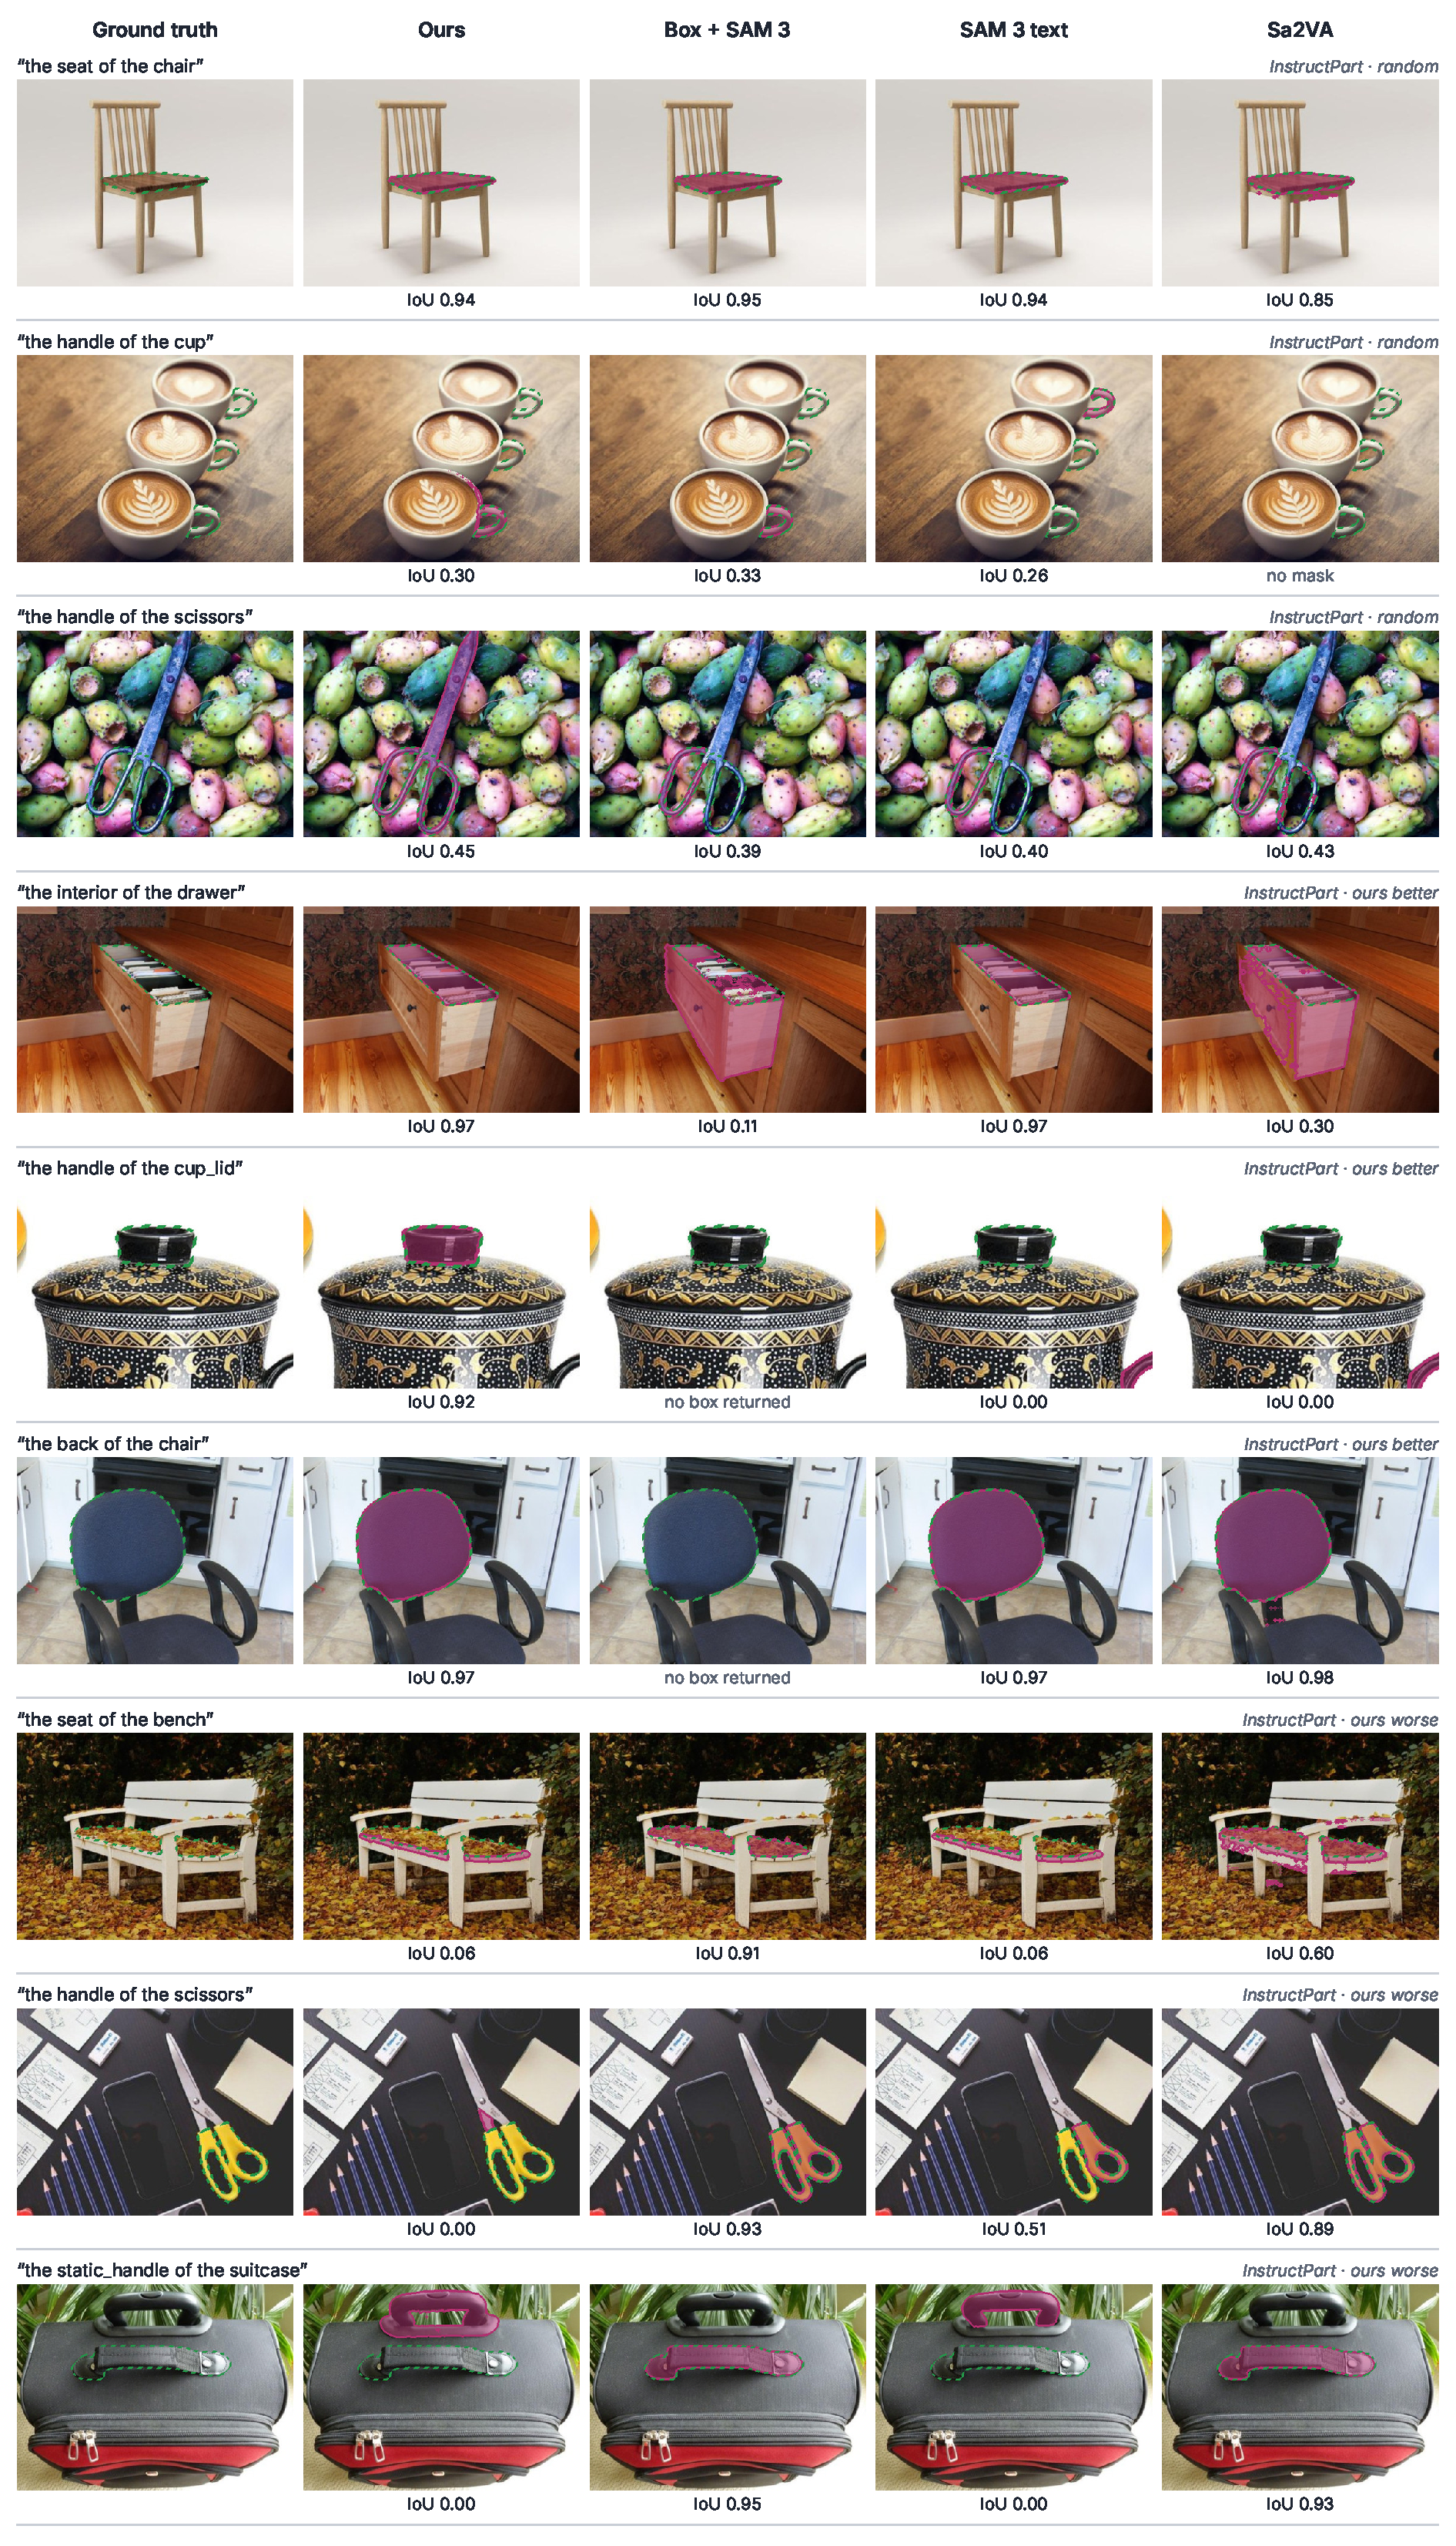
\includegraphics[width=\textwidth,height=0.92\textheight,keepaspectratio]{figures/qualitative/part_instructpart.pdf}
\caption{\textbf{Part grounding, InstructPart part names} (test). Rows: a fixed-seed random sample, the queries where \ours{} beats Box + SAM\,3 by the largest IoU margin, and those where it loses by the largest margin (labelled on each row).}
\label{fig:appx_part_instructpart}
\end{figure*}

\begin{figure*}[p]
\centering
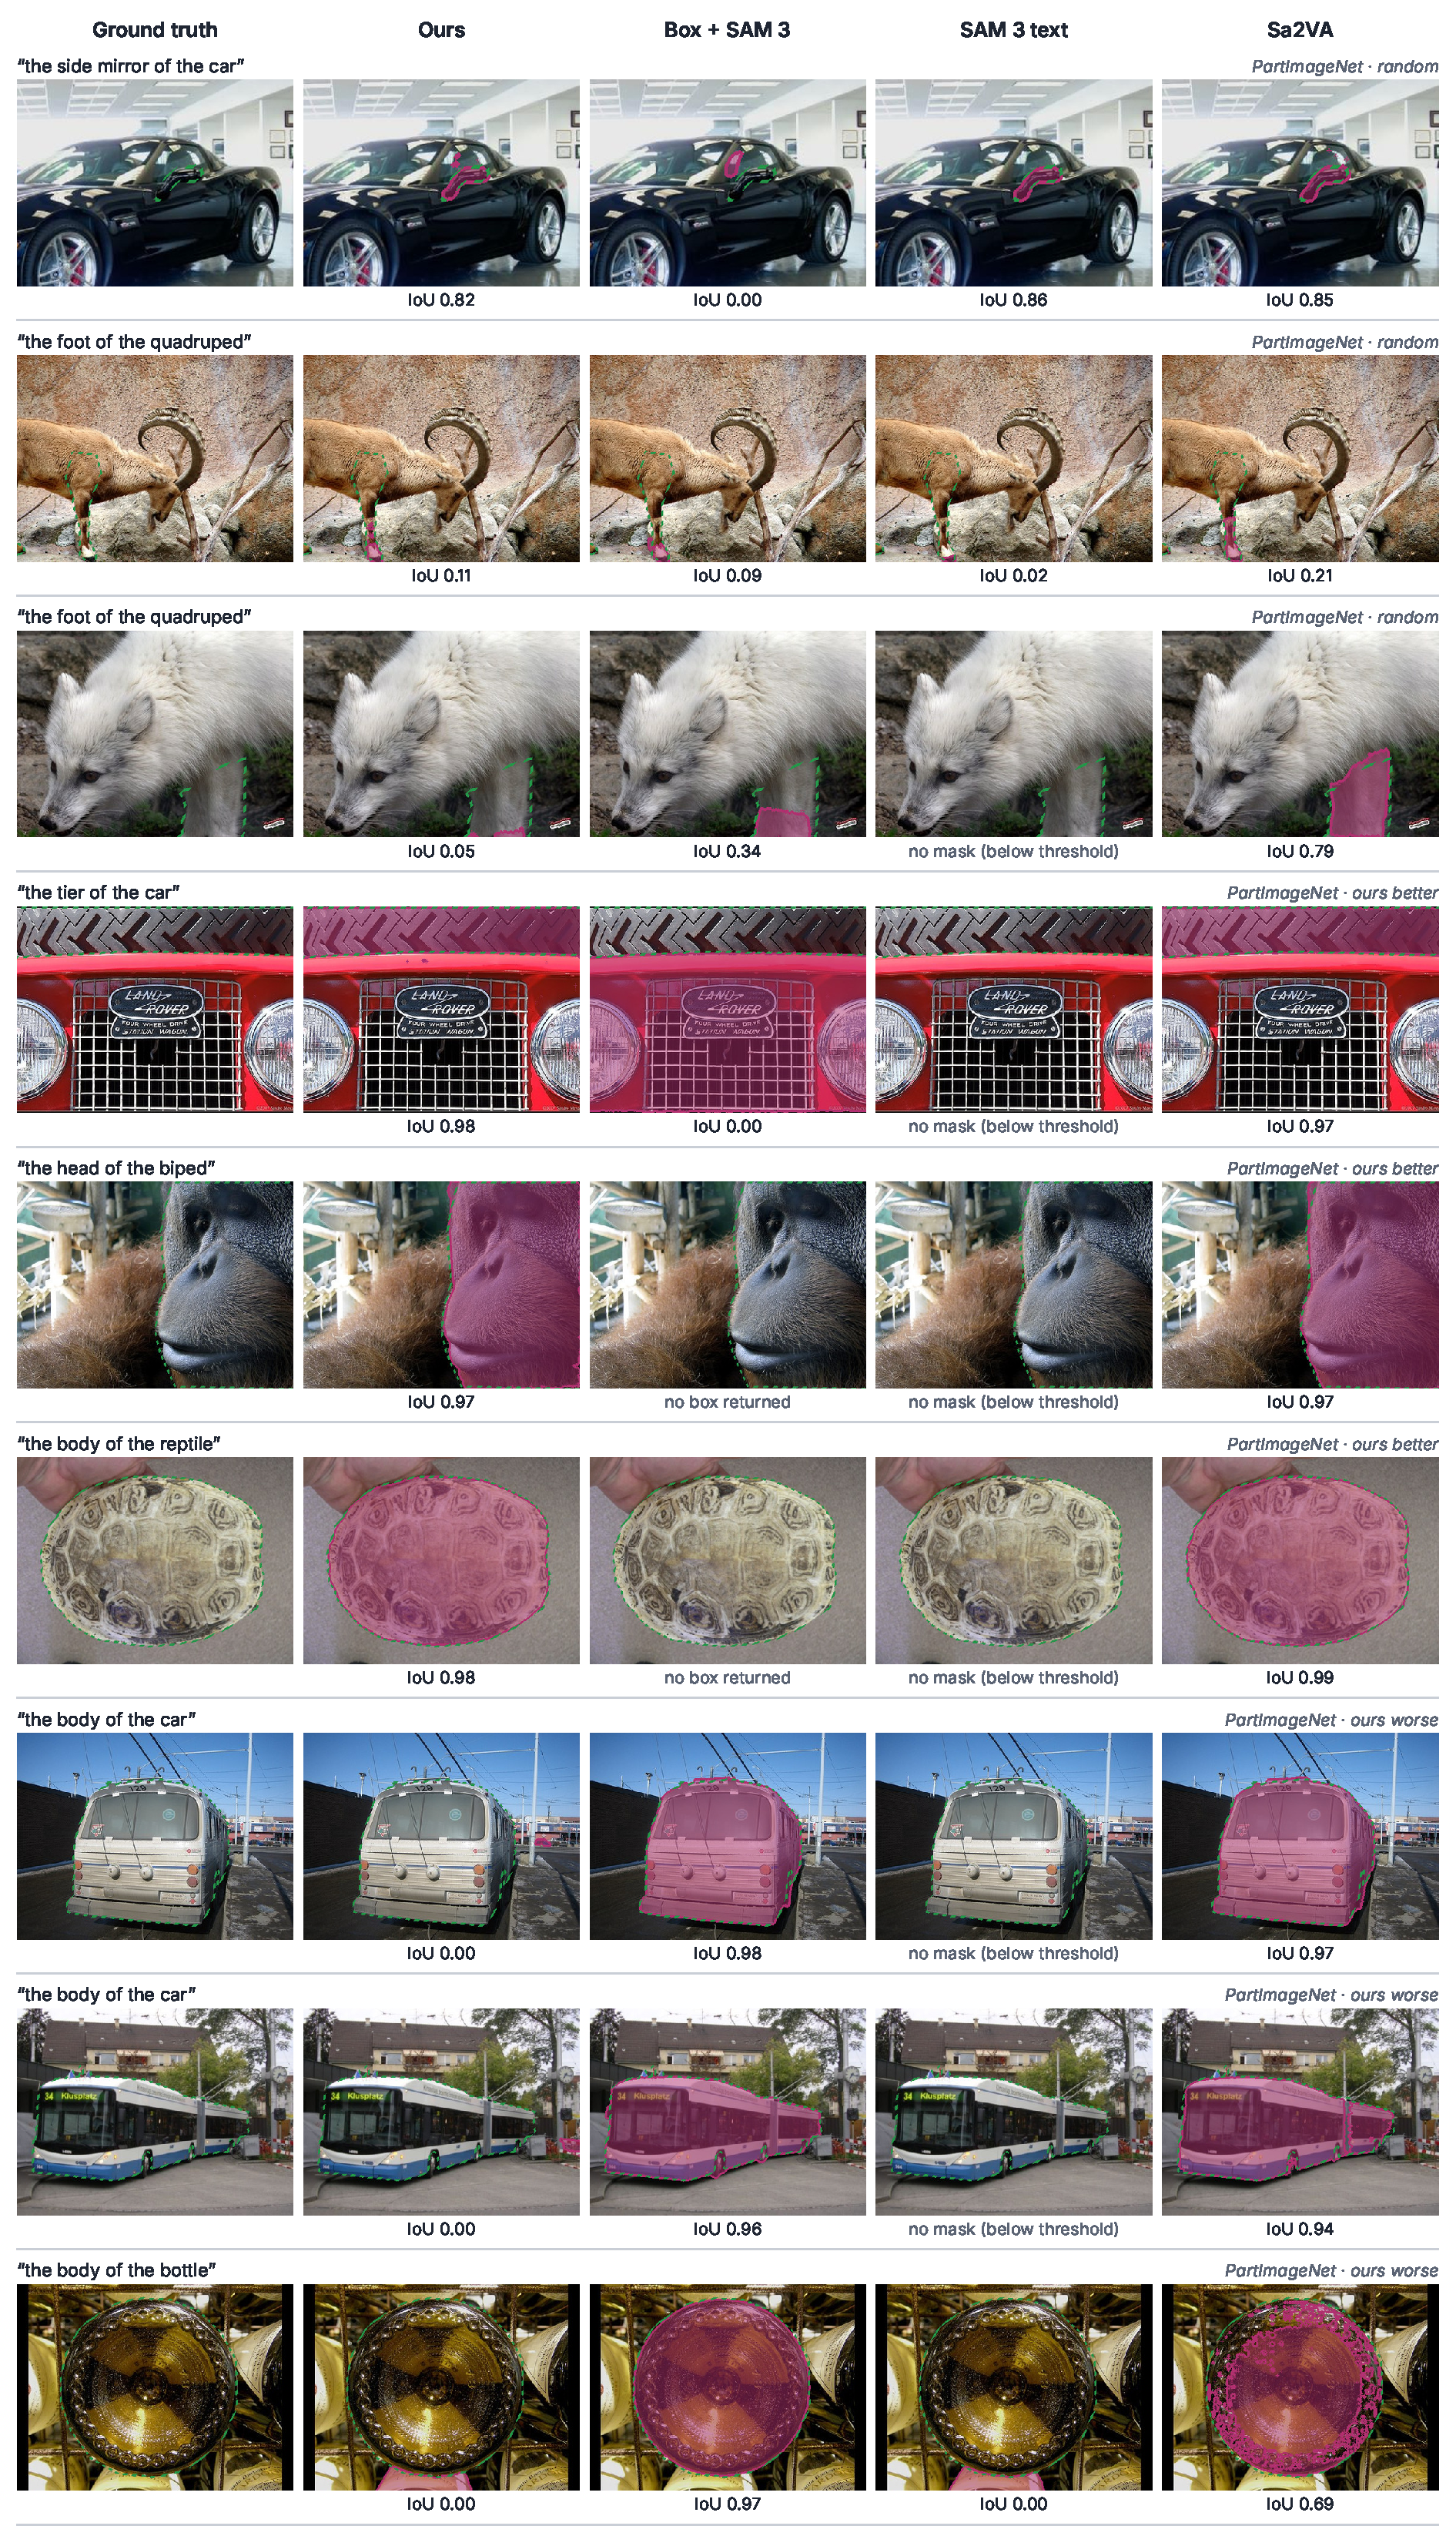
\includegraphics[width=\textwidth,height=0.92\textheight,keepaspectratio]{figures/qualitative/part_partimagenet.pdf}
\caption{\textbf{Part grounding, PartImageNet} (test). Rows: a fixed-seed random sample, the queries where \ours{} beats Box + SAM\,3 by the largest IoU margin, and those where it loses by the largest margin (labelled on each row).}
\label{fig:appx_part_partimagenet}
\end{figure*}

\begin{figure*}[p]
\centering
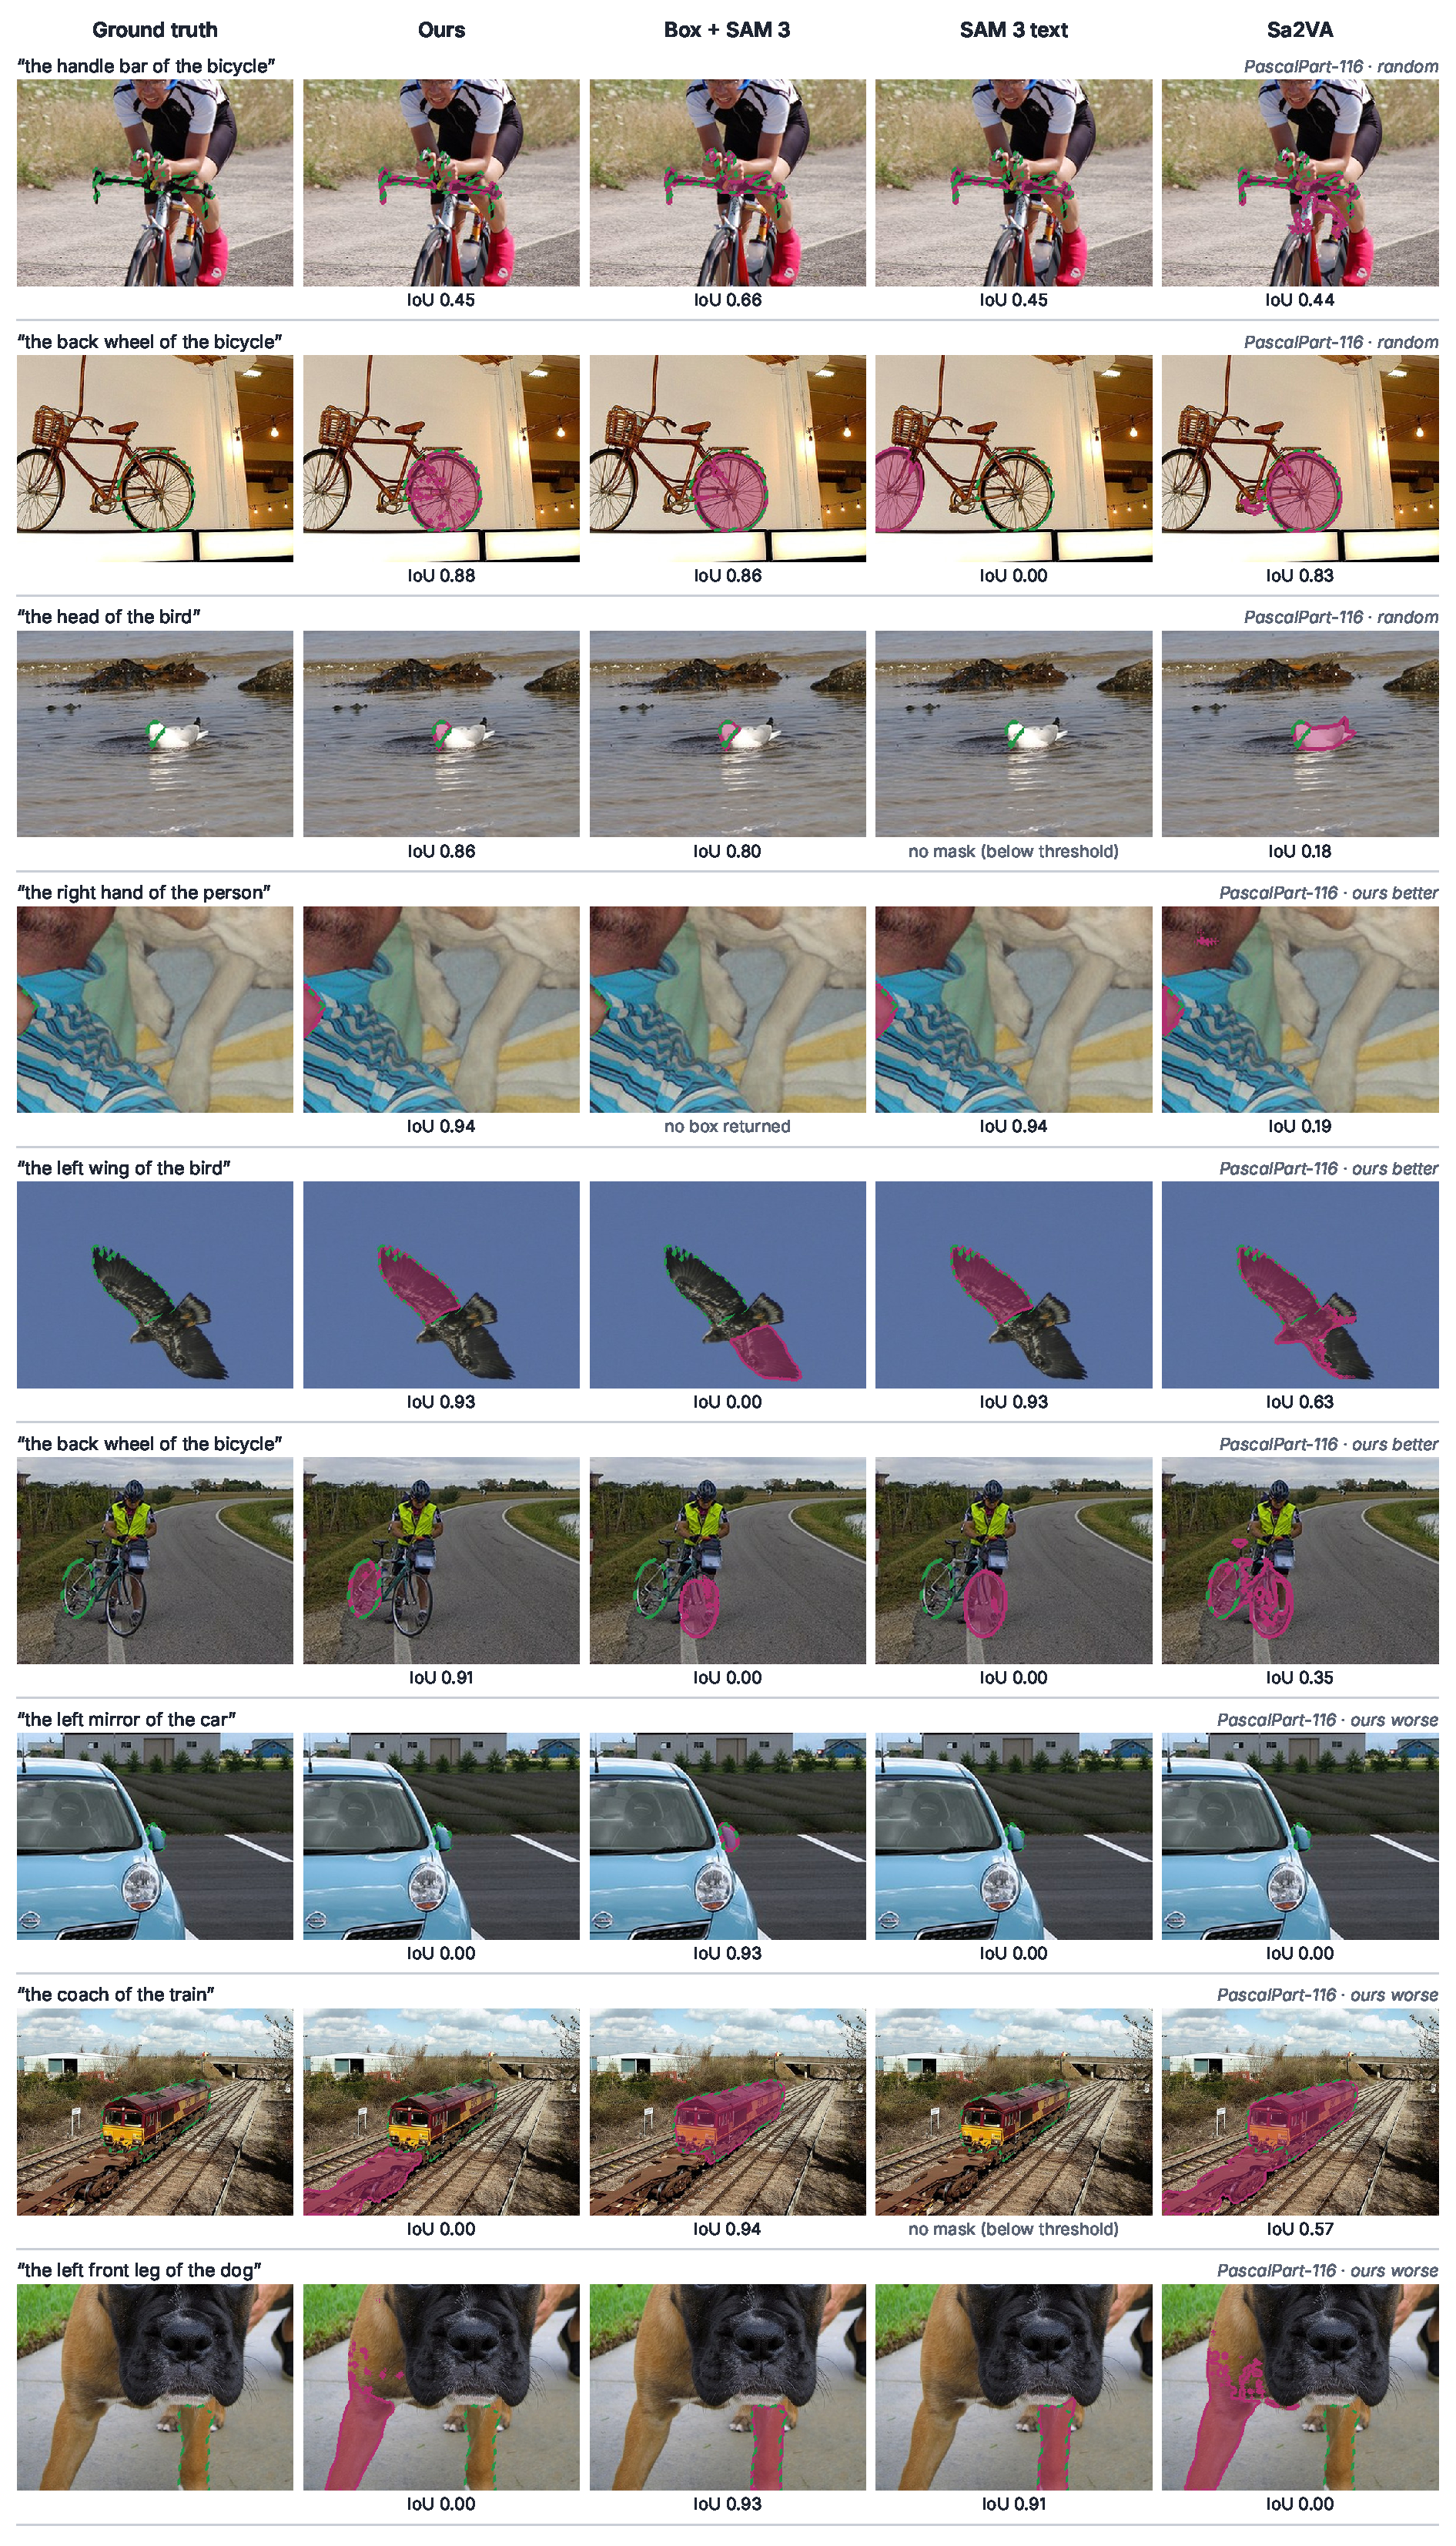
\includegraphics[width=\textwidth,height=0.92\textheight,keepaspectratio]{figures/qualitative/part_pascalpart.pdf}
\caption{\textbf{Part grounding, PascalPart-116} (test). Rows: a fixed-seed random sample, the queries where \ours{} beats Box + SAM\,3 by the largest IoU margin, and those where it loses by the largest margin (labelled on each row).}
\label{fig:appx_part_pascalpart}
\end{figure*}

\begin{figure*}[p]
\centering
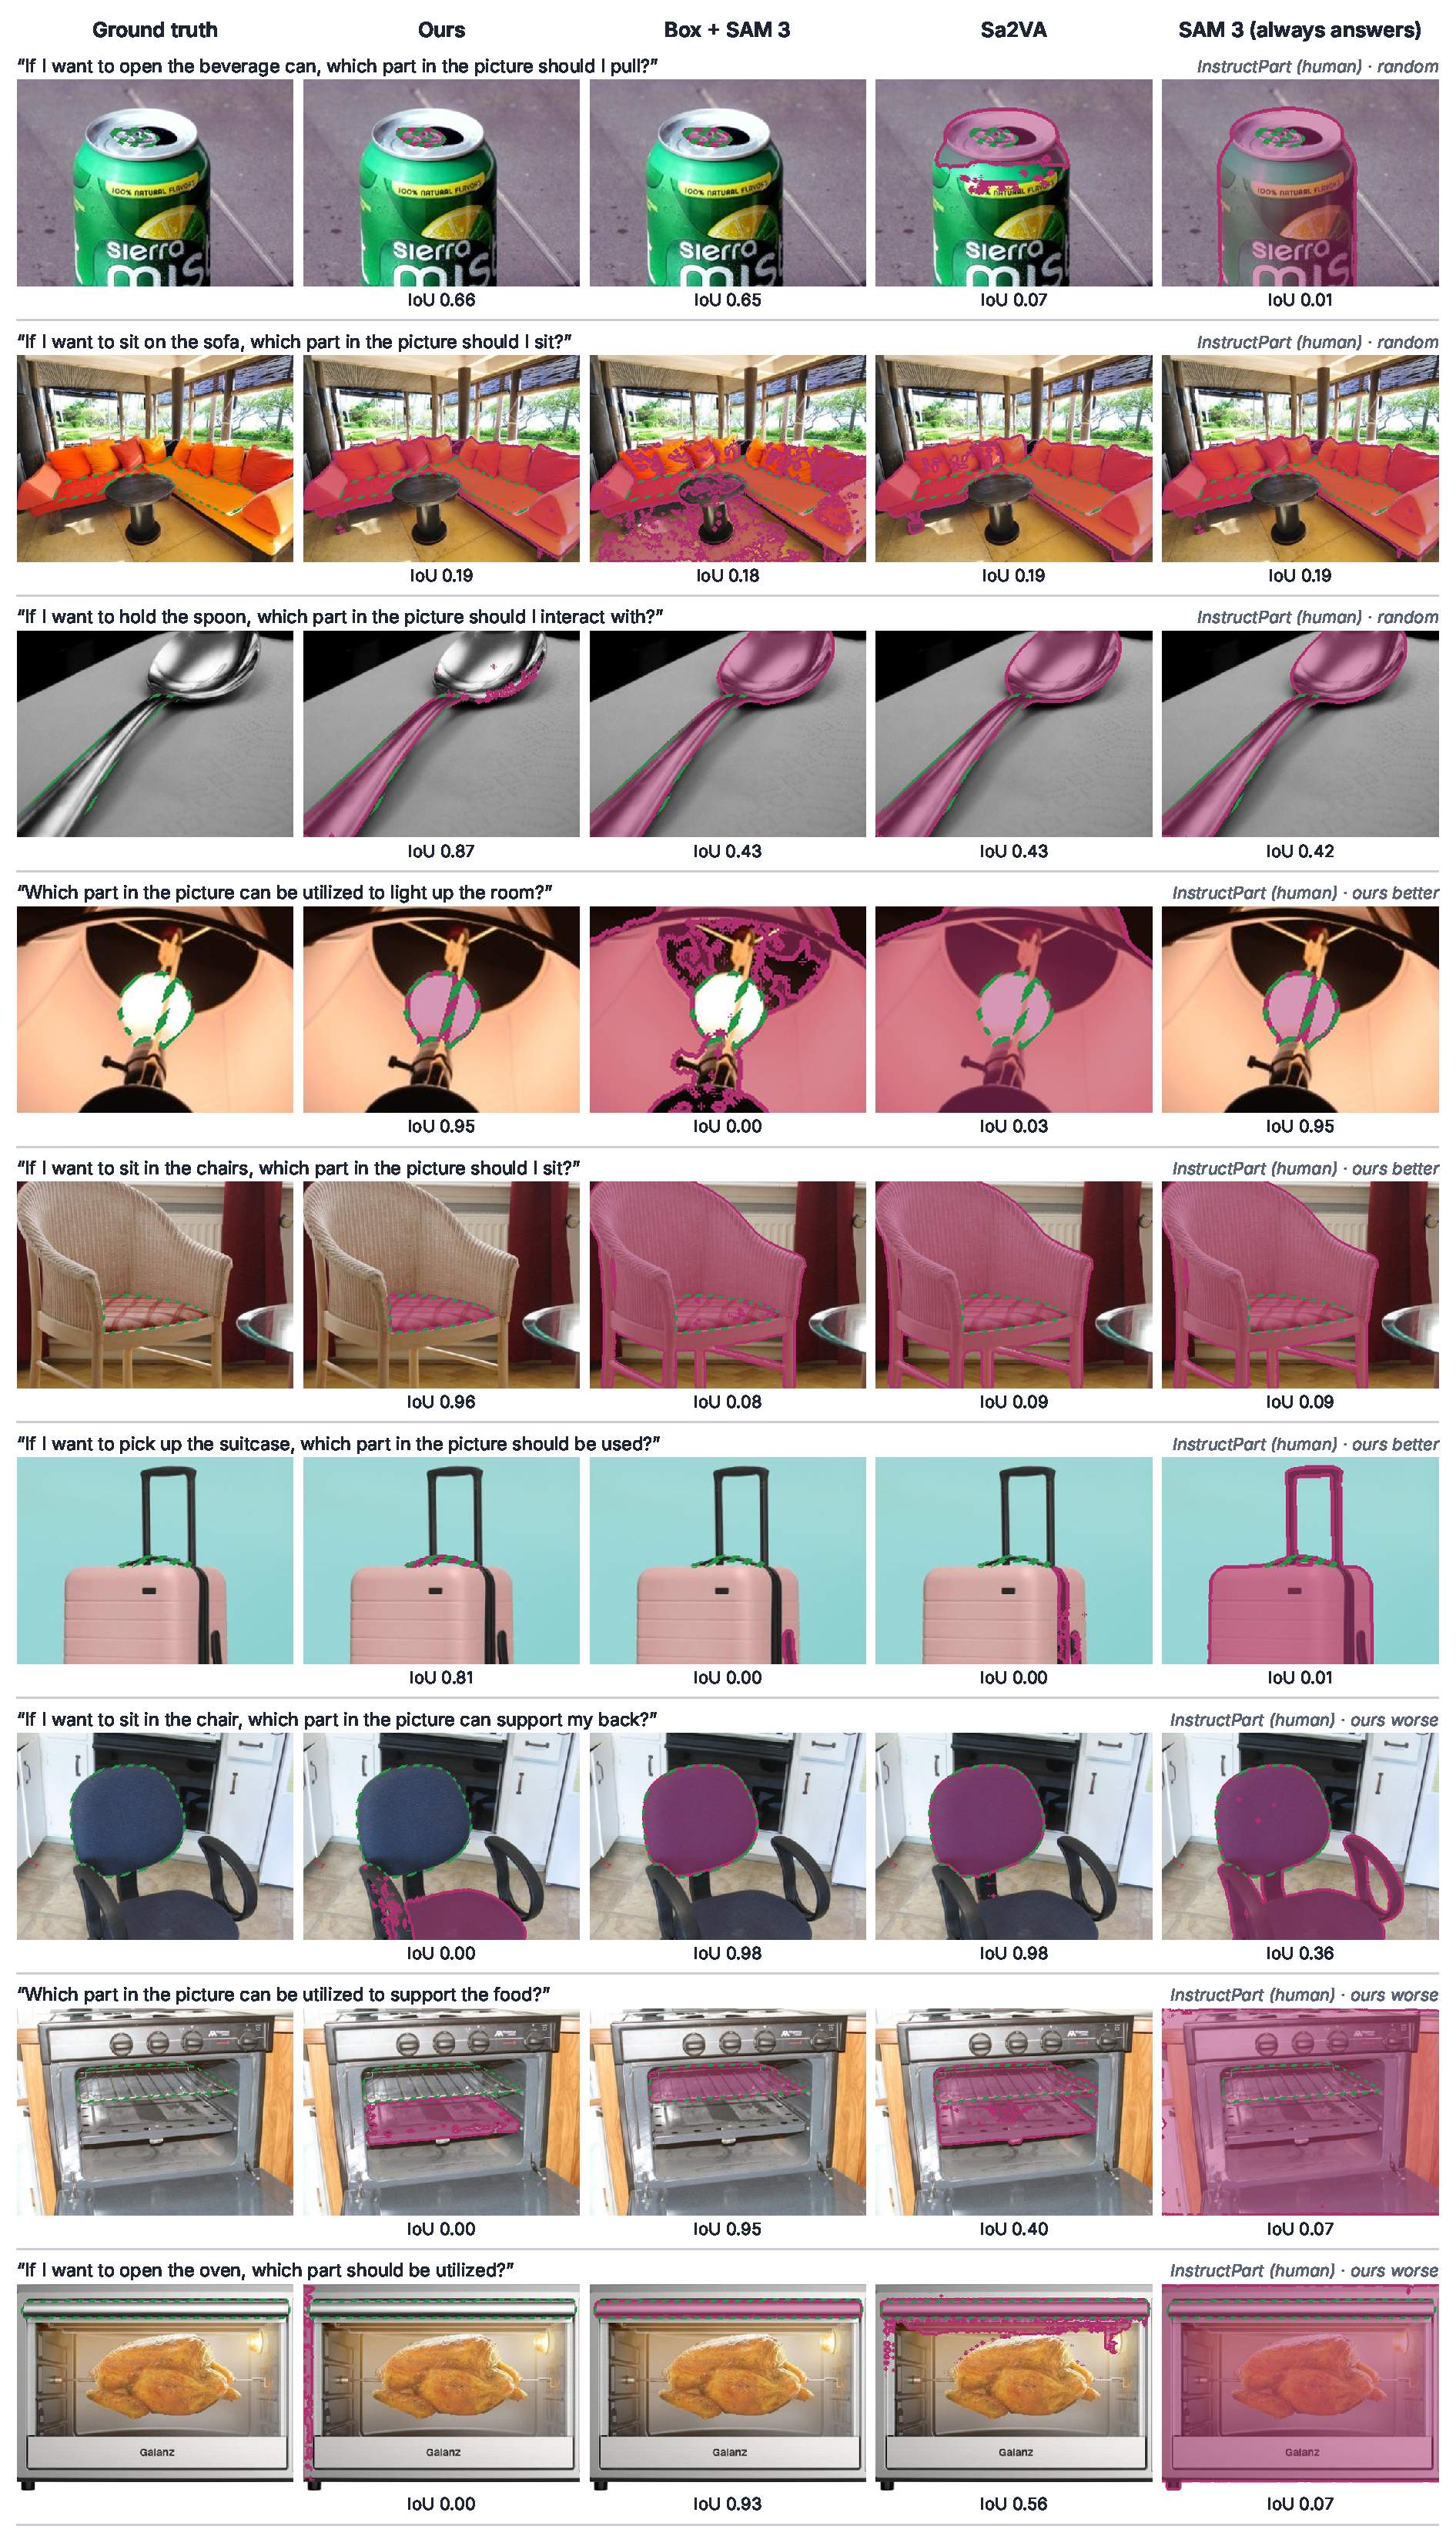
\includegraphics[width=\textwidth,height=0.92\textheight,keepaspectratio]{figures/qualitative/reason_instructpart_human.pdf}
\caption{\textbf{Reasoning, InstructPart human-written instructions} (test; \ours{} without query rewriting). Rows: a fixed-seed random sample, the queries where \ours{} beats Box + SAM\,3 by the largest IoU margin, and those where it loses by the largest margin (labelled on each row).}
\label{fig:appx_reason_instructpart_human}
\end{figure*}

\begin{figure*}[p]
\centering
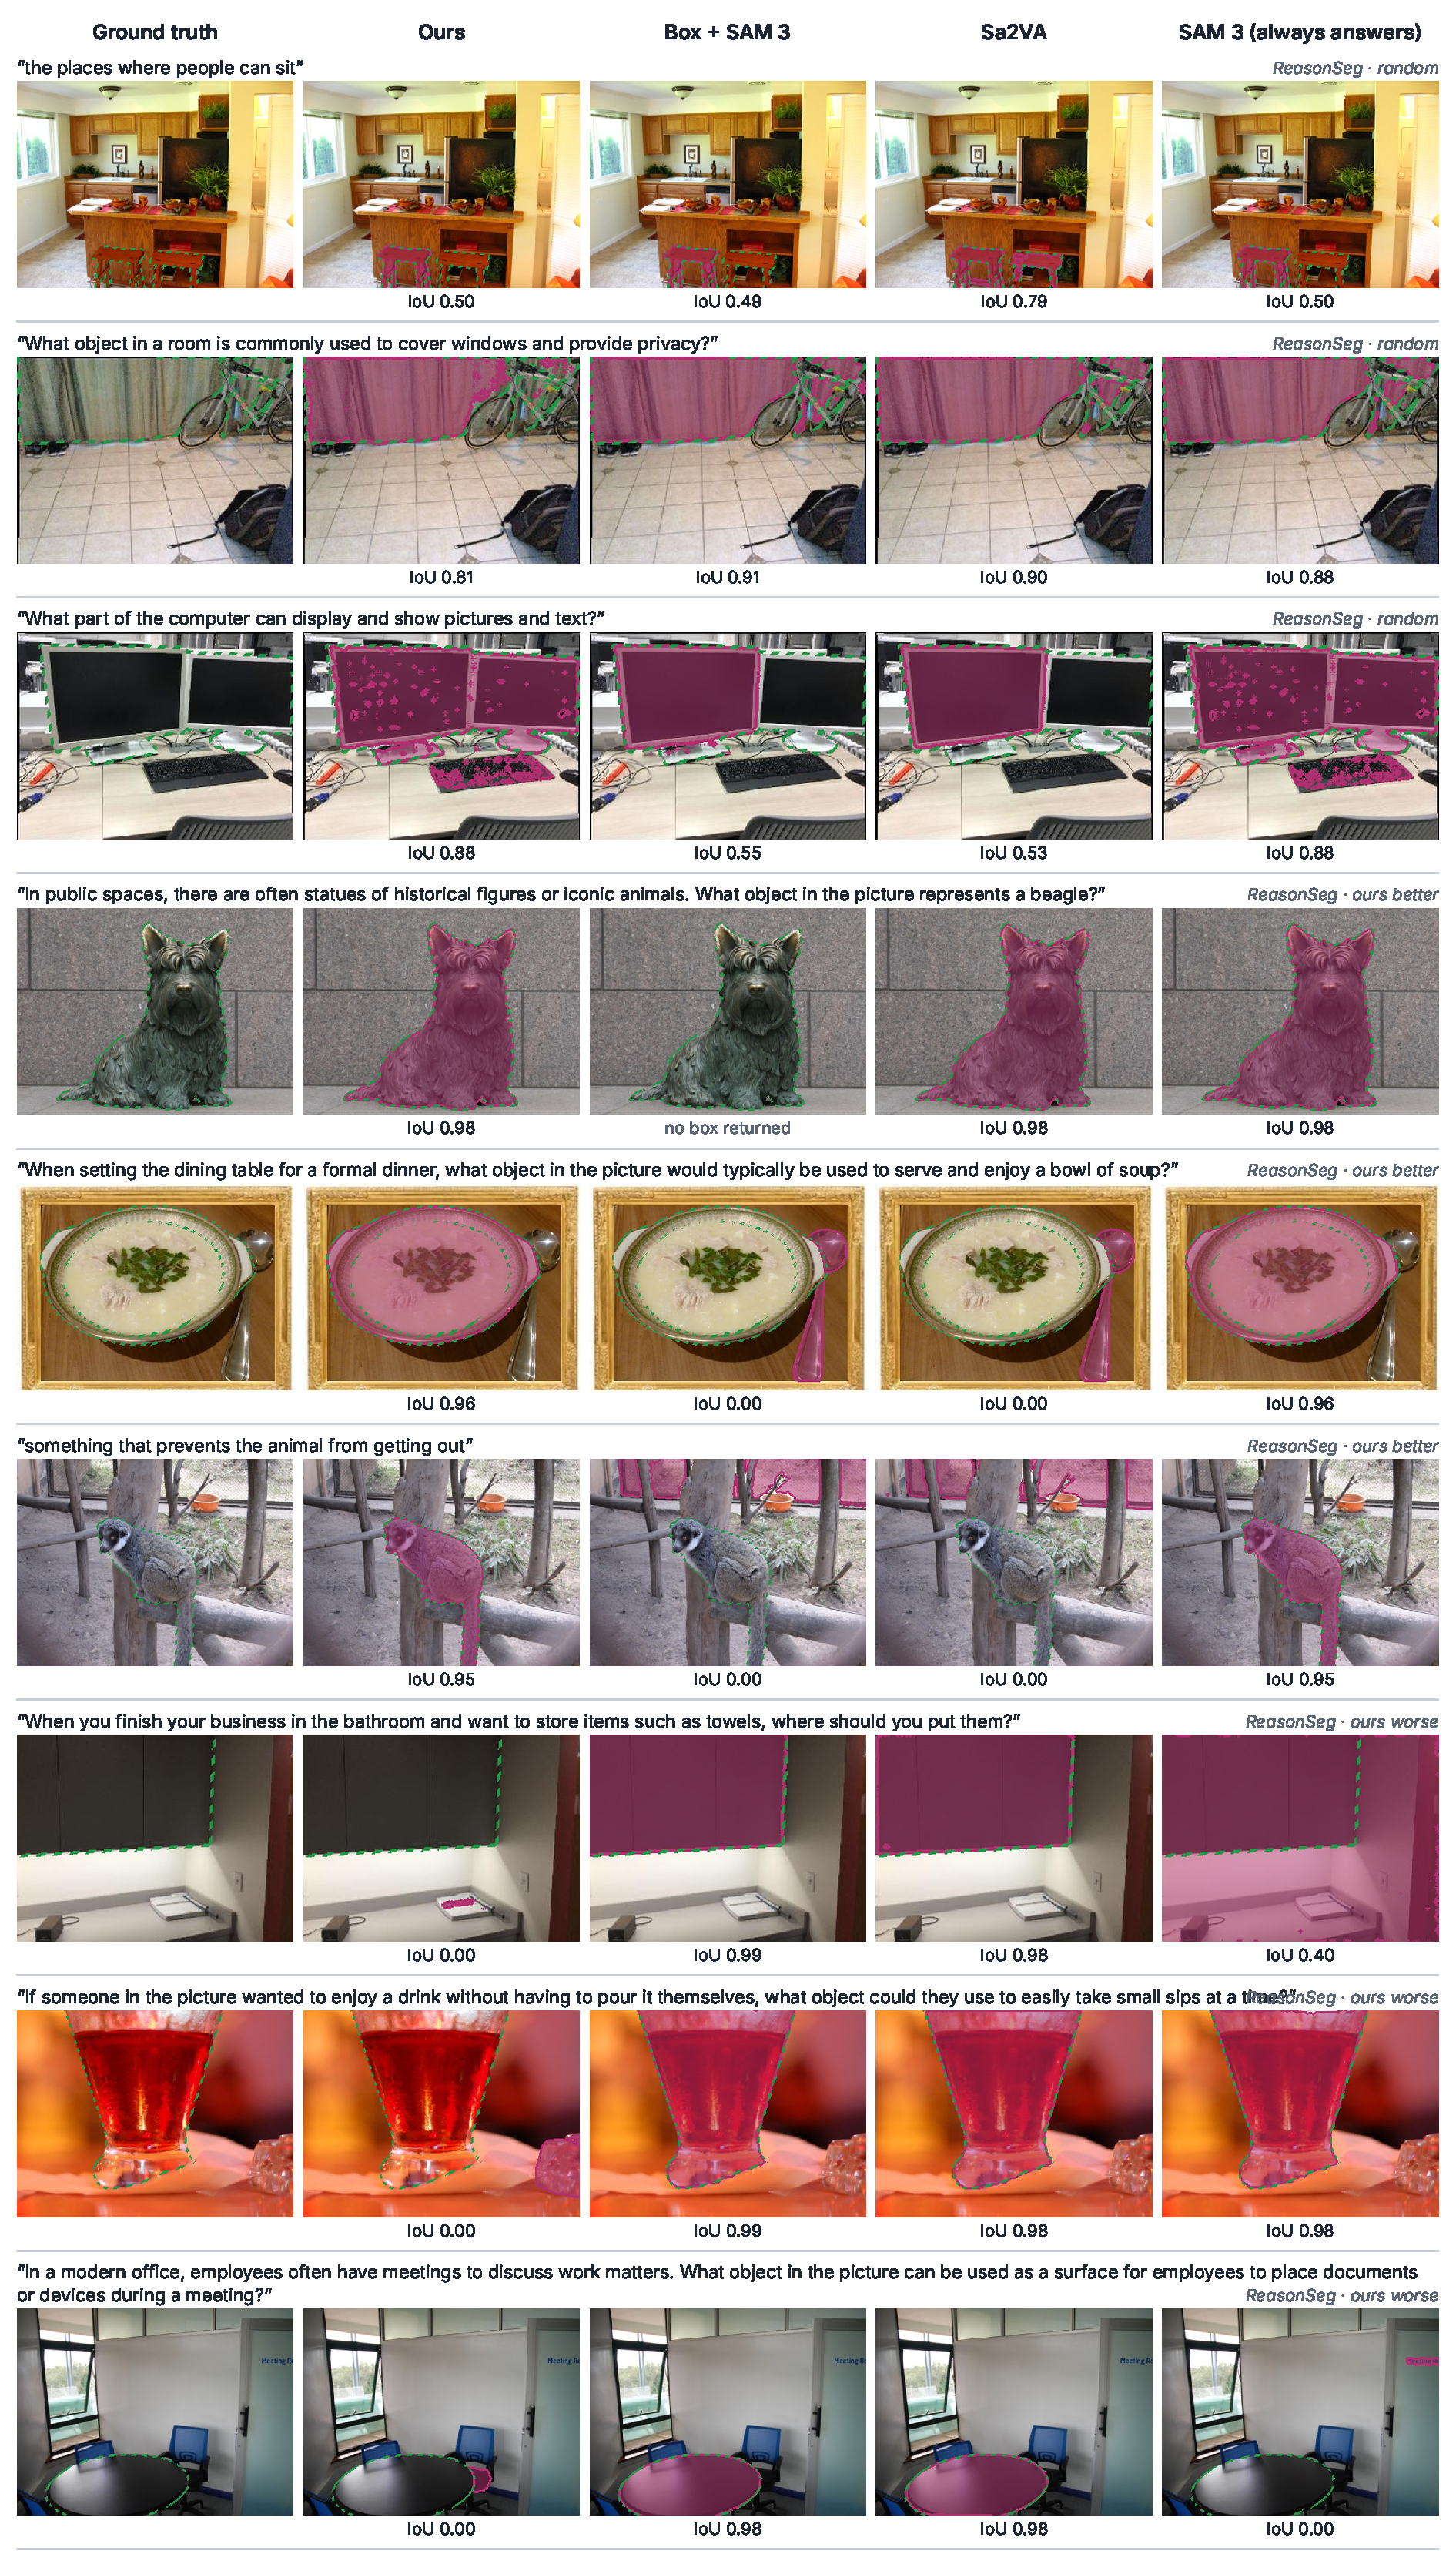
\includegraphics[width=\textwidth,height=0.92\textheight,keepaspectratio]{figures/qualitative/reason_reasonseg.pdf}
\caption{\textbf{Reasoning, ReasonSeg} (test; \ours{} without query rewriting). Rows: a fixed-seed random sample, the queries where \ours{} beats Box + SAM\,3 by the largest IoU margin, and those where it loses by the largest margin (labelled on each row).}
\label{fig:appx_reason_reasonseg}
\end{figure*}

\begin{figure*}[p]
\centering
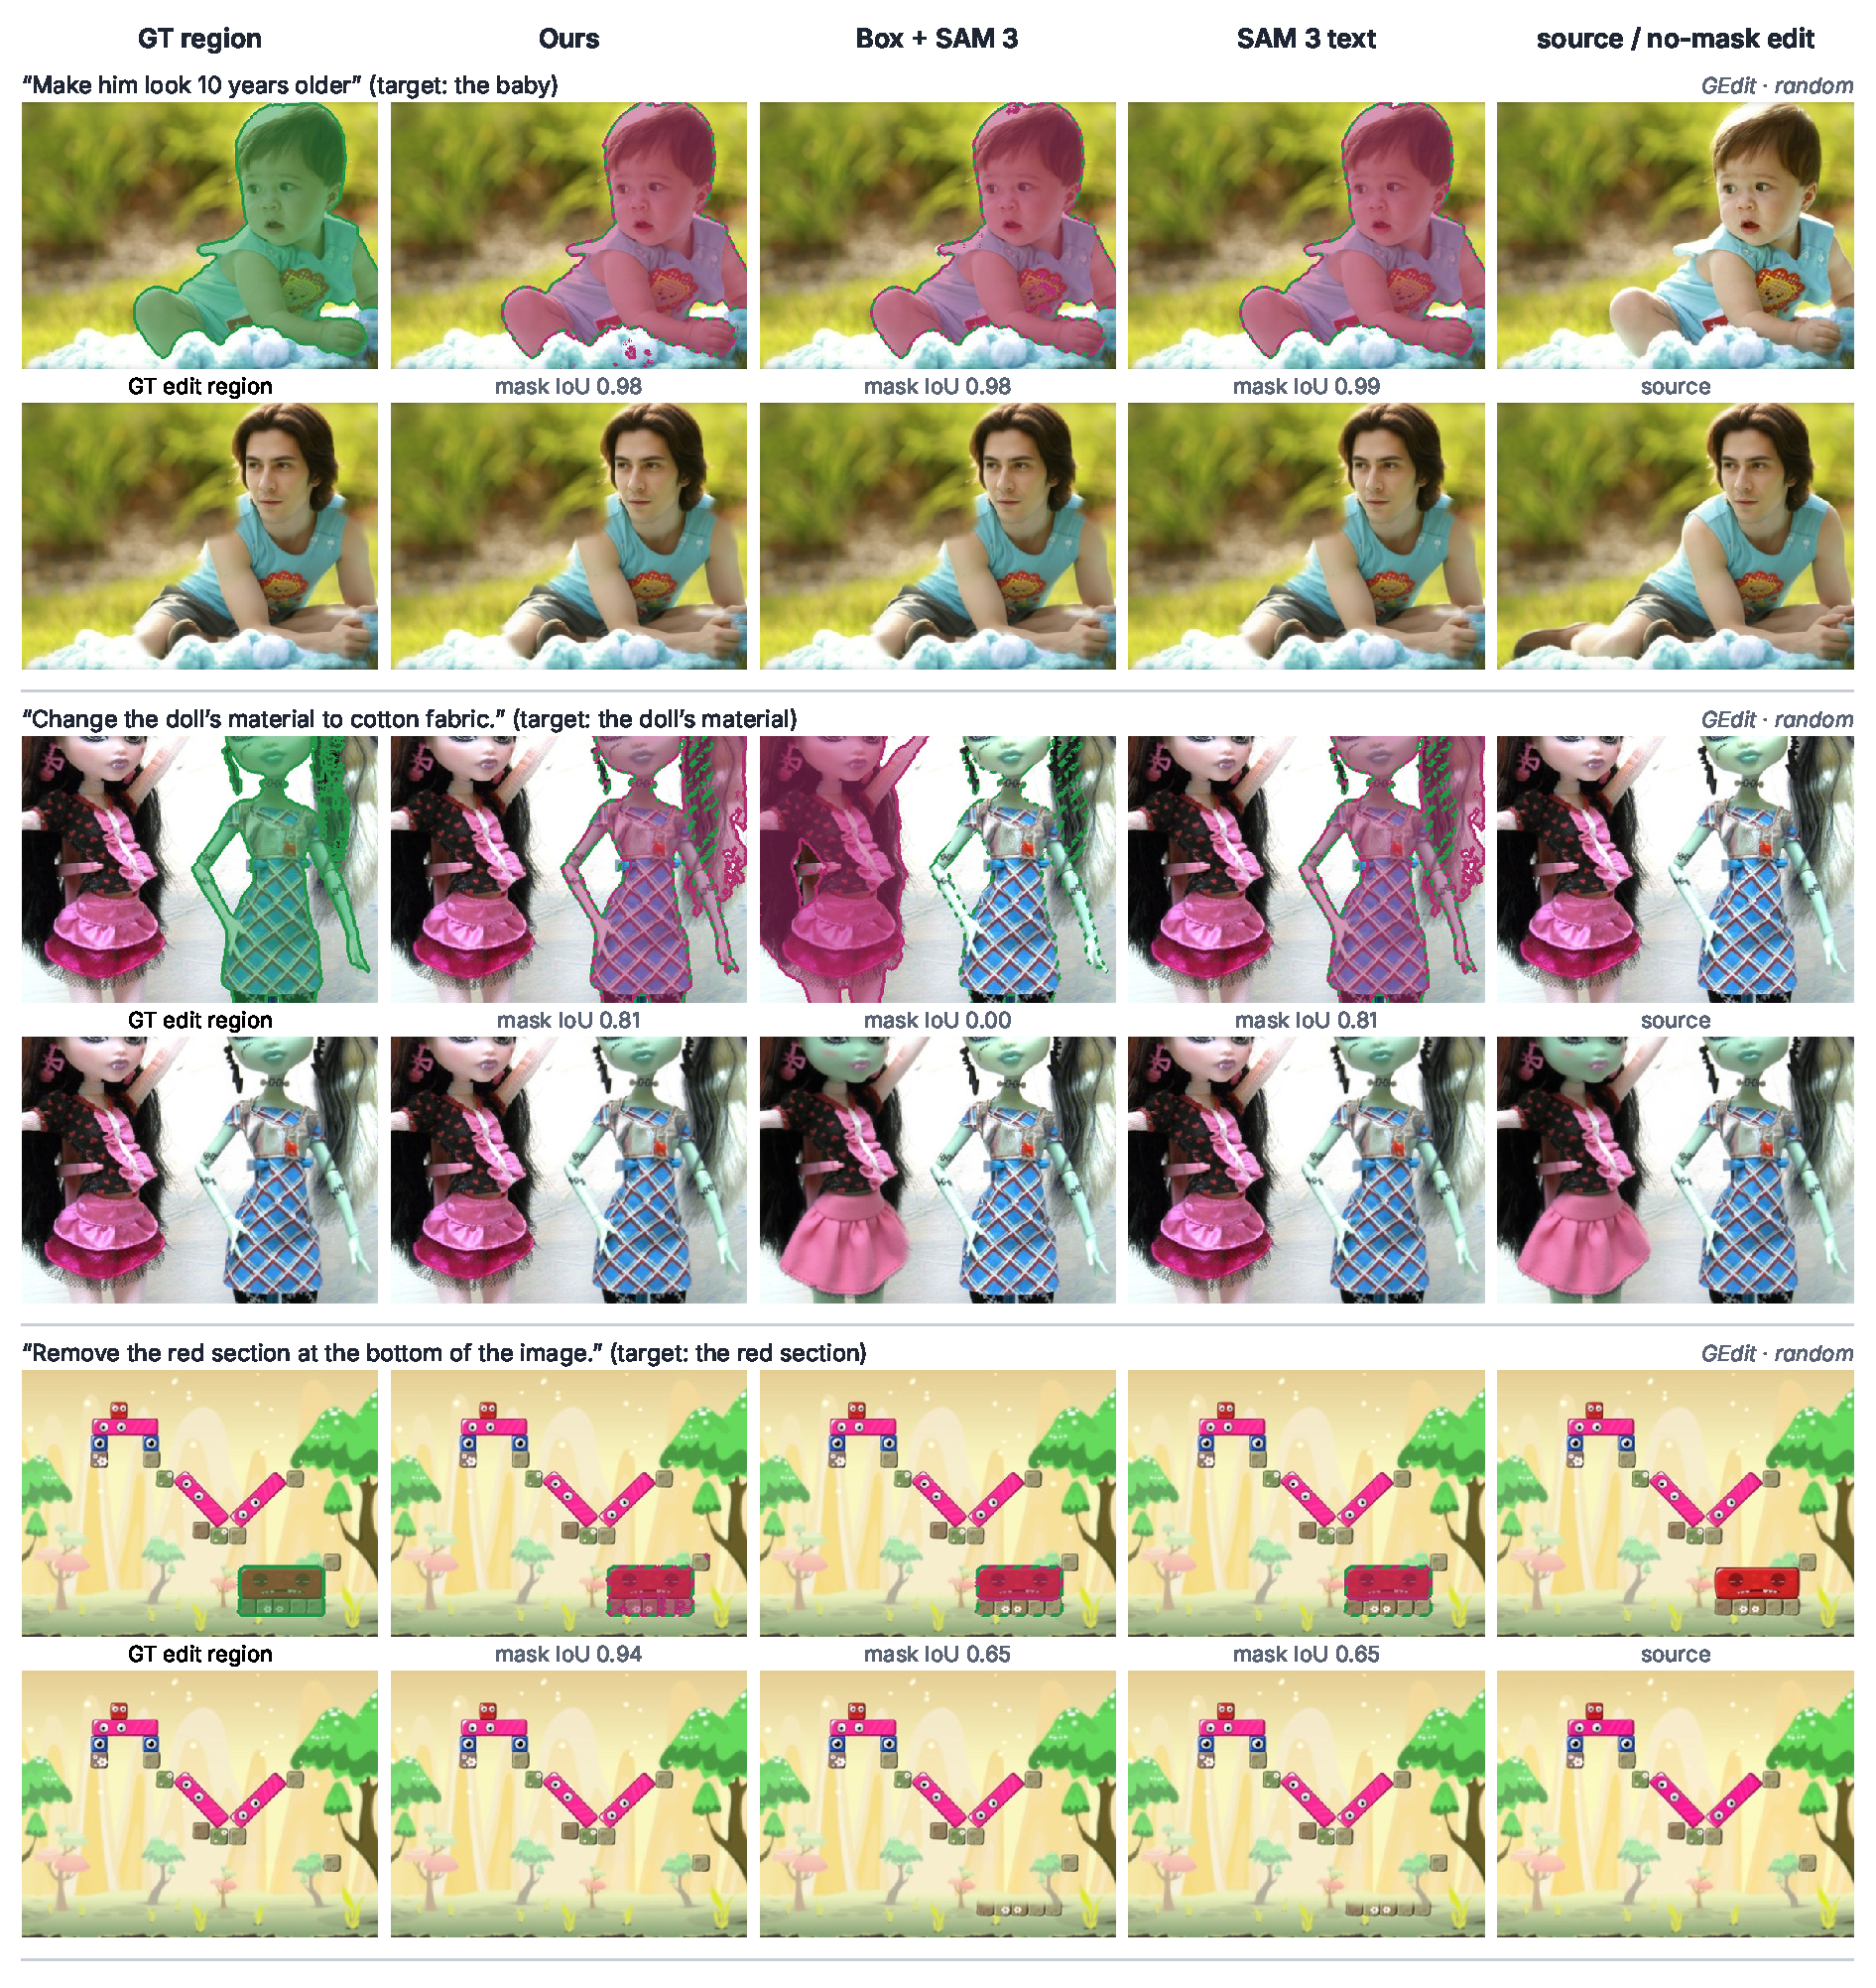
\includegraphics[width=\textwidth,height=0.92\textheight,keepaspectratio]{figures/qualitative/edit_gedit_random.pdf}
\caption{\textbf{Editing, GEdit-Bench-EN, Qwen-Image-Edit, random sample.} Top: masks of each source (GT edit region dashed); bottom: the edit within each mask and the unmasked edit.}
\label{fig:appx_edit_gedit_random}
\end{figure*}

\begin{figure*}[p]
\centering
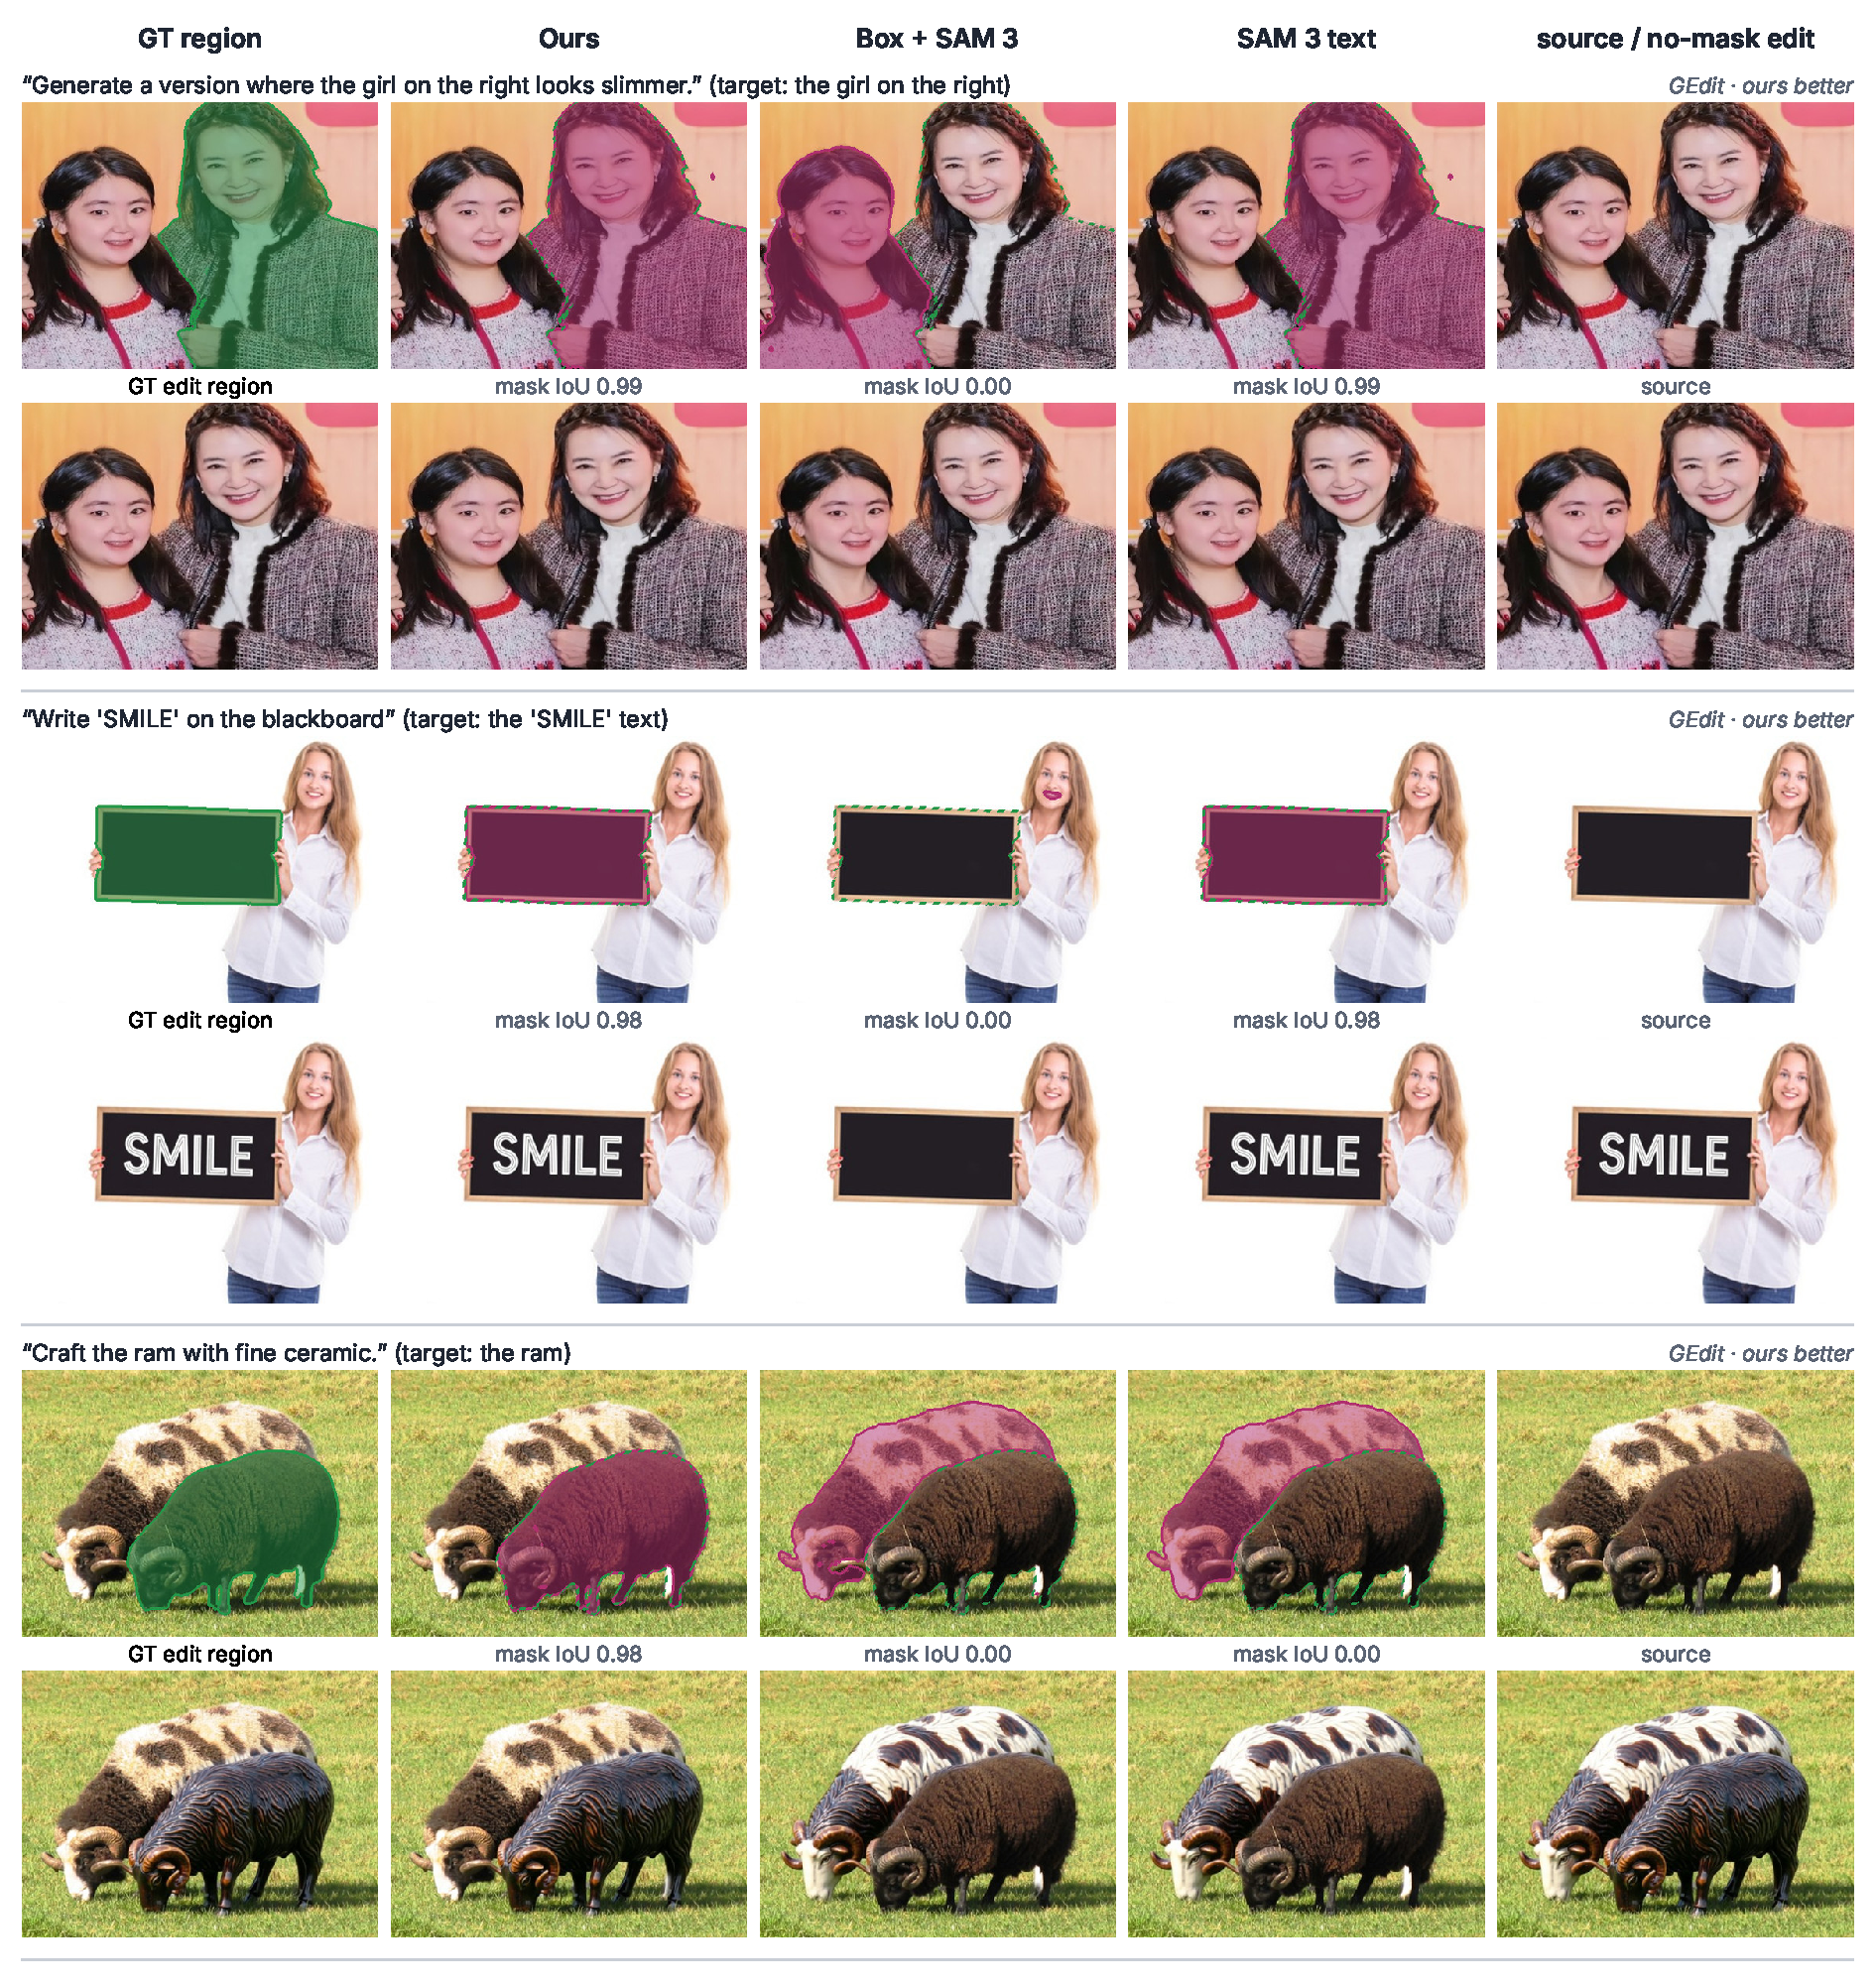
\includegraphics[width=\textwidth,height=0.92\textheight,keepaspectratio]{figures/qualitative/edit_gedit_ours_better.pdf}
\caption{\textbf{Editing, GEdit-Bench-EN, Qwen-Image-Edit, largest margins for \ours{}.} Top: masks of each source (GT edit region dashed); bottom: the edit within each mask and the unmasked edit.}
\label{fig:appx_edit_gedit_ours_better}
\end{figure*}

\begin{figure*}[p]
\centering
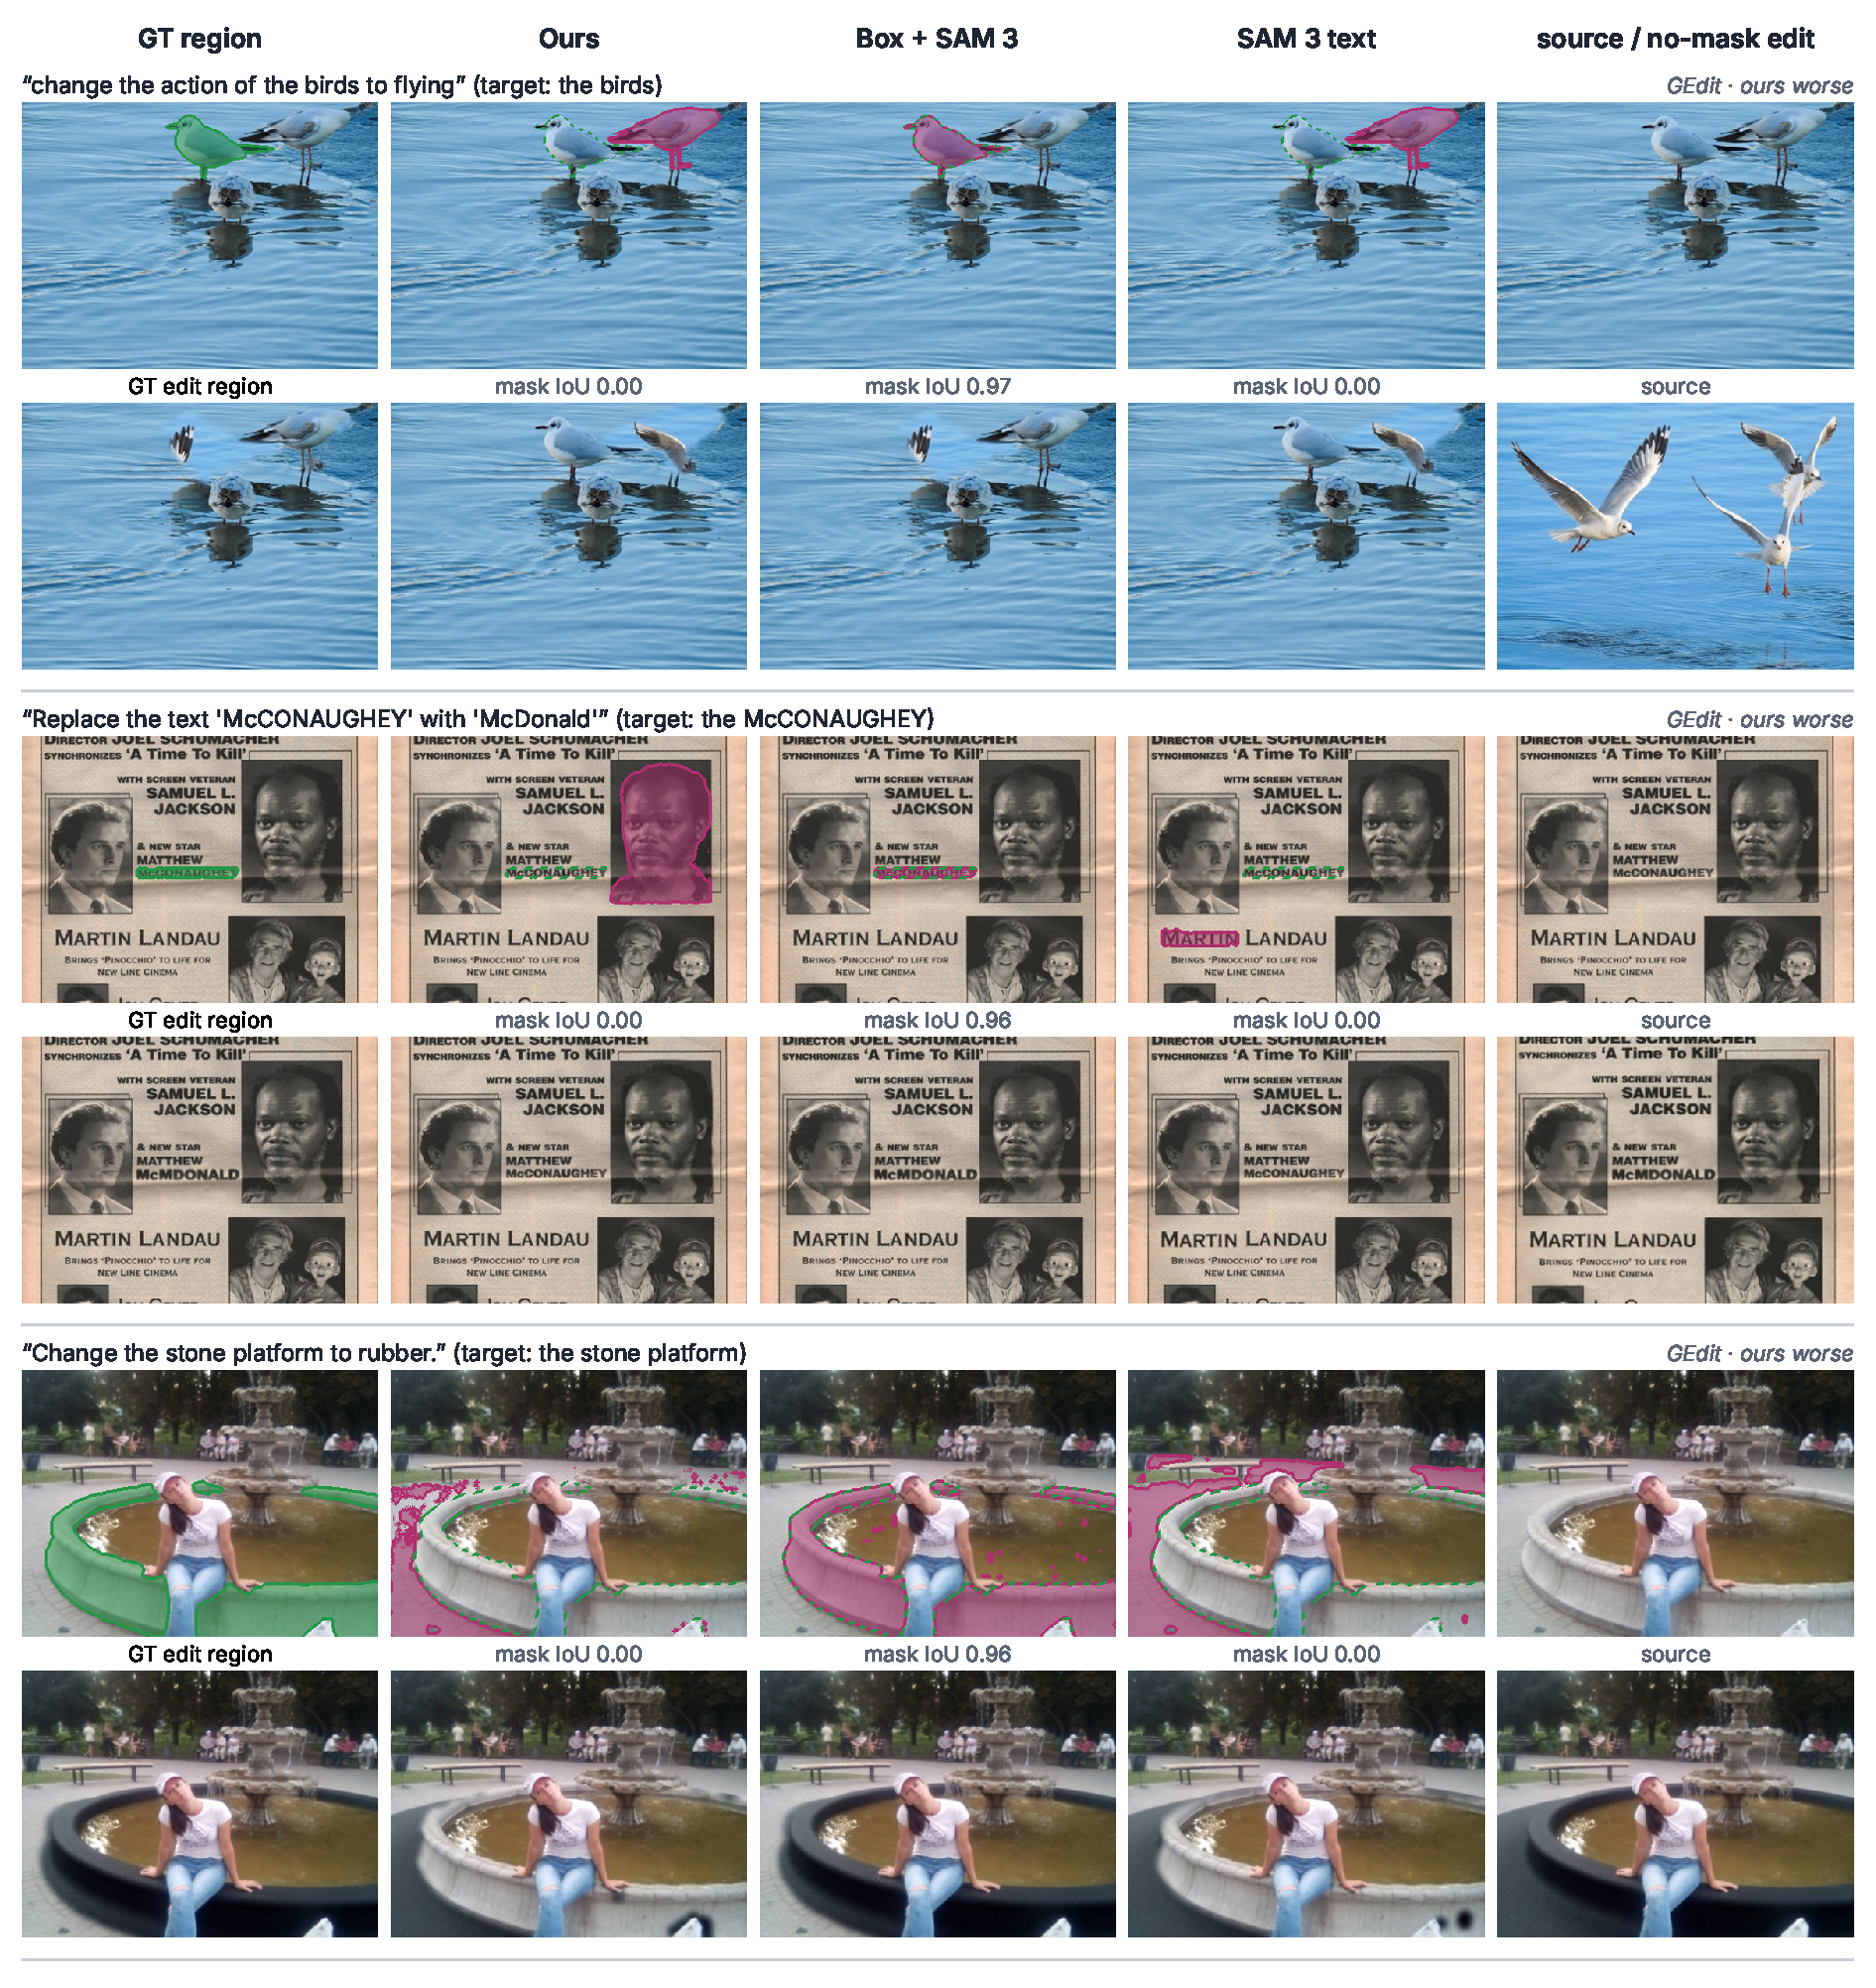
\includegraphics[width=\textwidth,height=0.92\textheight,keepaspectratio]{figures/qualitative/edit_gedit_ours_worse.pdf}
\caption{\textbf{Editing, GEdit-Bench-EN, Qwen-Image-Edit, largest margins against \ours{}.} Top: masks of each source (GT edit region dashed); bottom: the edit within each mask and the unmasked edit.}
\label{fig:appx_edit_gedit_ours_worse}
\end{figure*}

\begin{figure*}[p]
\centering
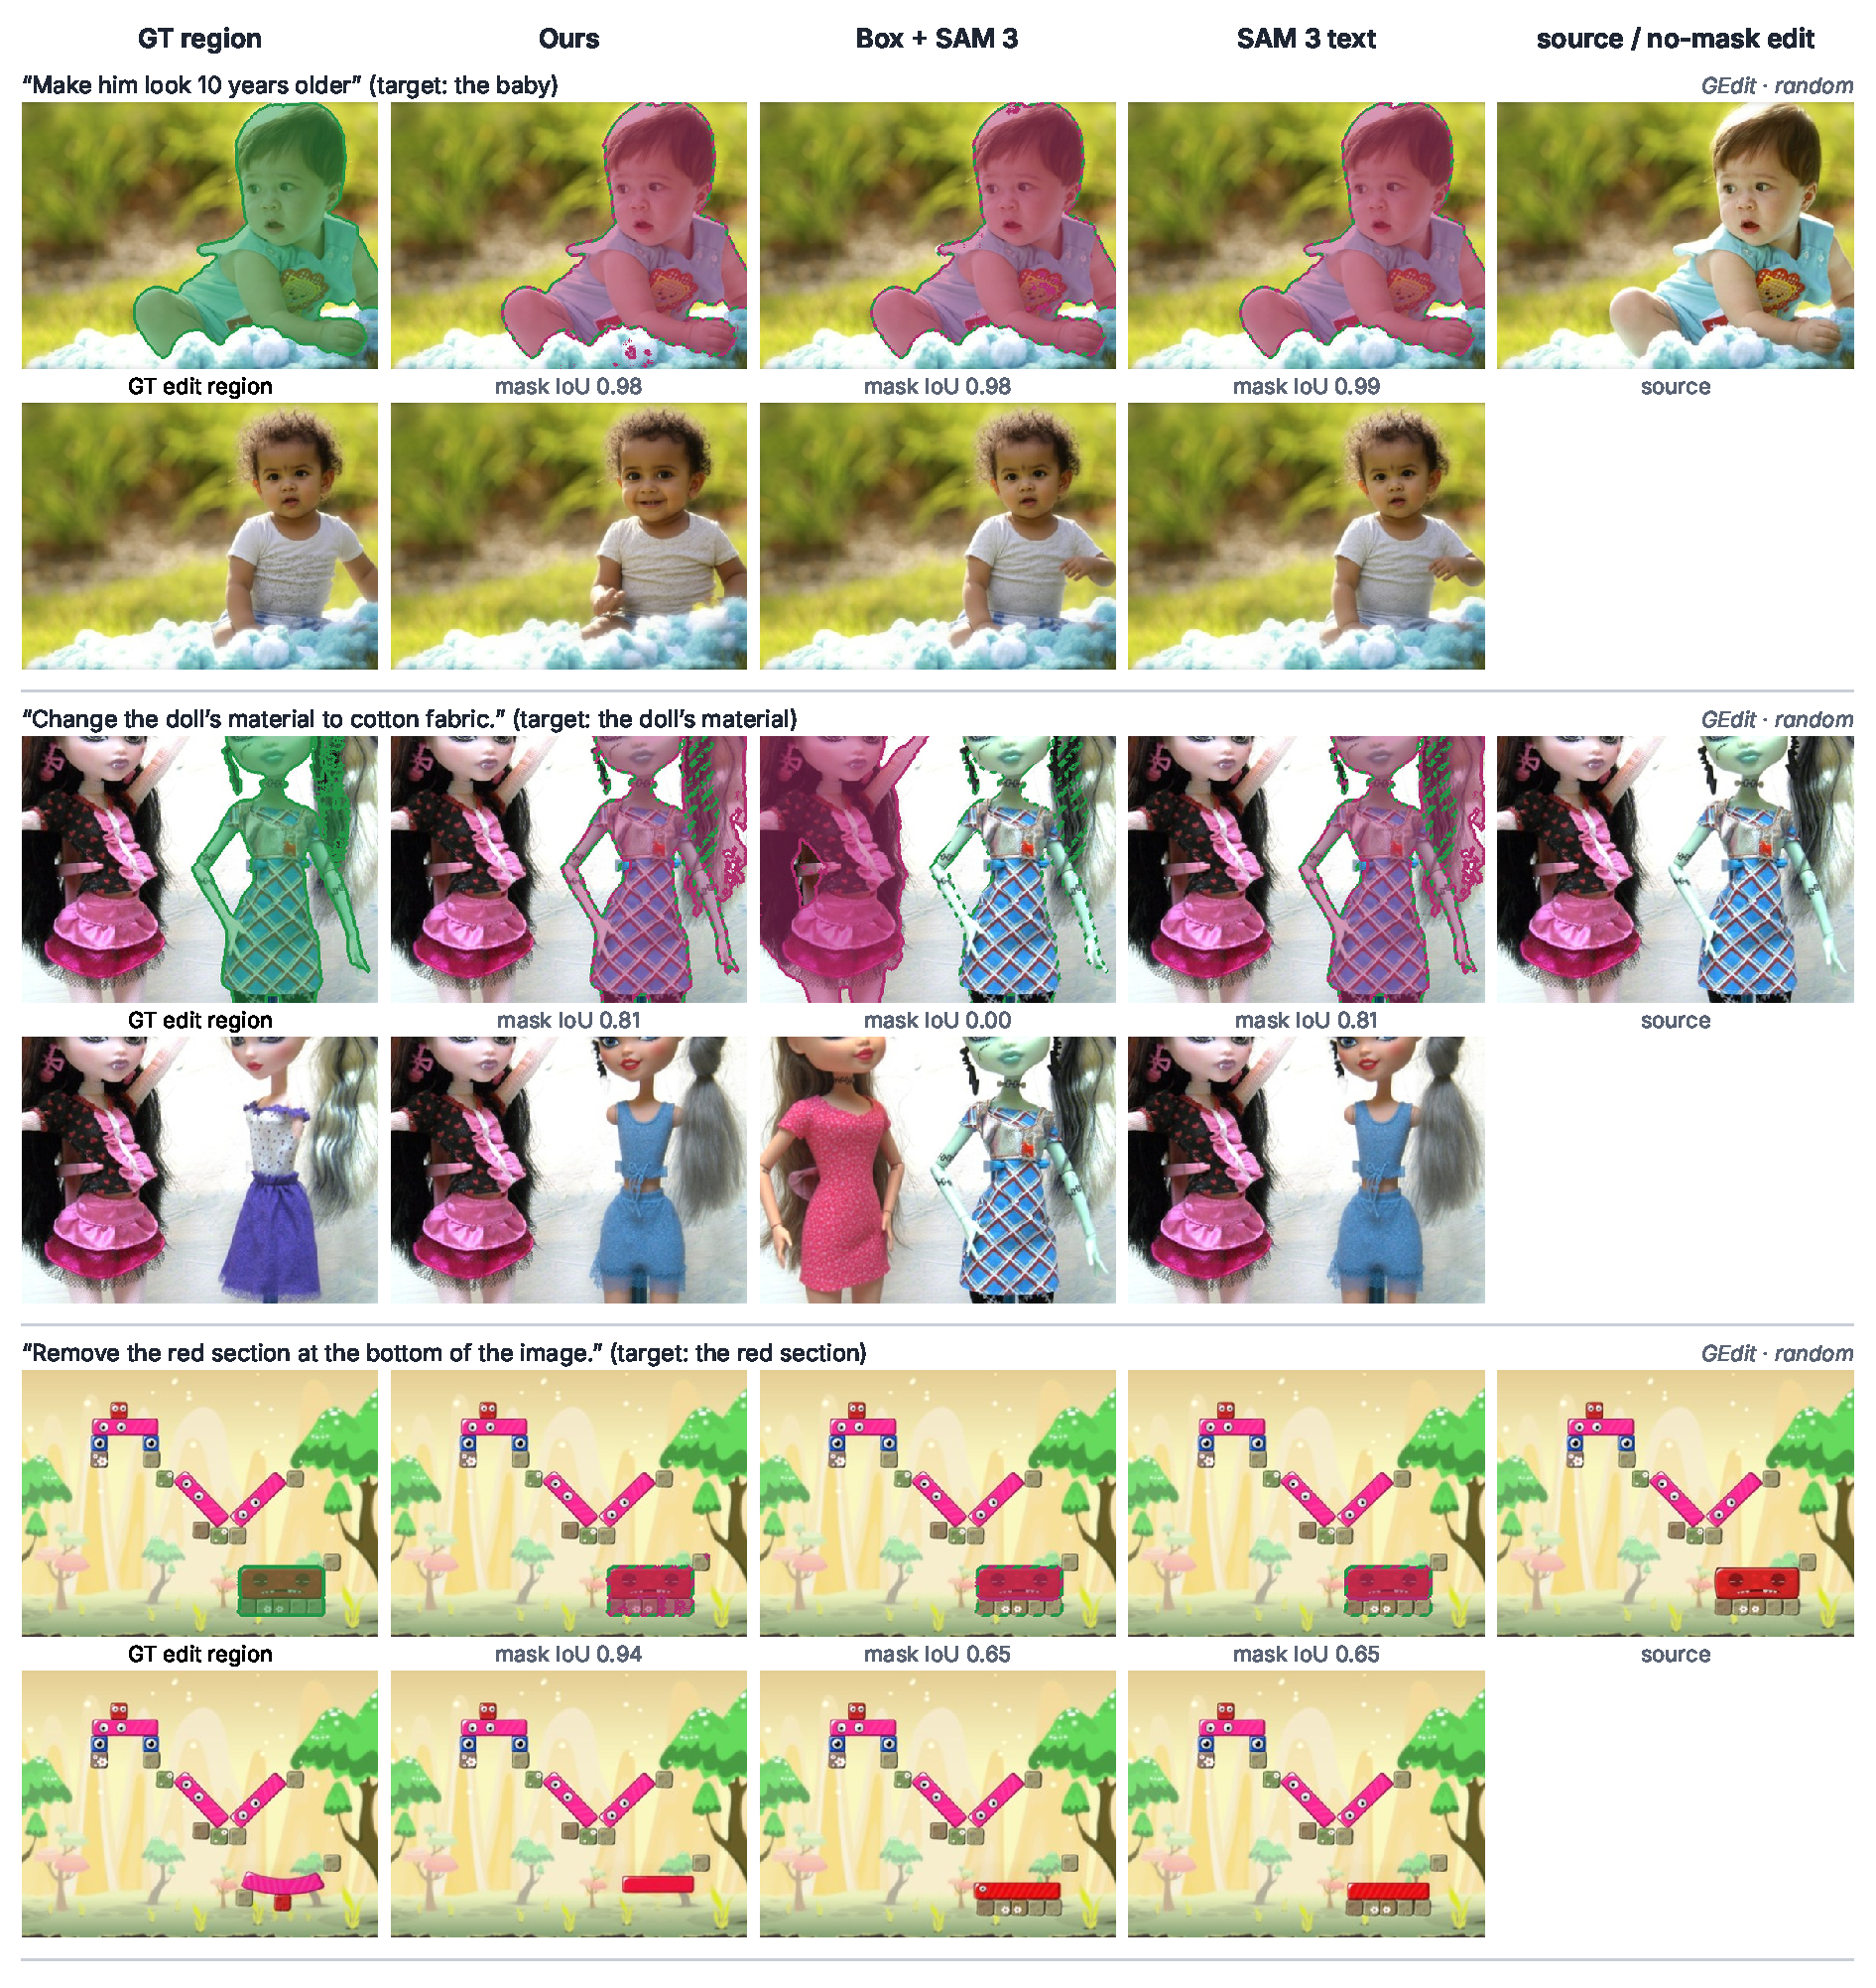
\includegraphics[width=\textwidth,height=0.92\textheight,keepaspectratio]{figures/qualitative/edit_gedit_random_flux.pdf}
\caption{\textbf{Editing, GEdit-Bench-EN, FLUX Fill, random sample.} As above, with FLUX Fill inpainting each mask.}
\label{fig:appx_edit_gedit_flux}
\end{figure*}

\begin{figure*}[p]
\centering
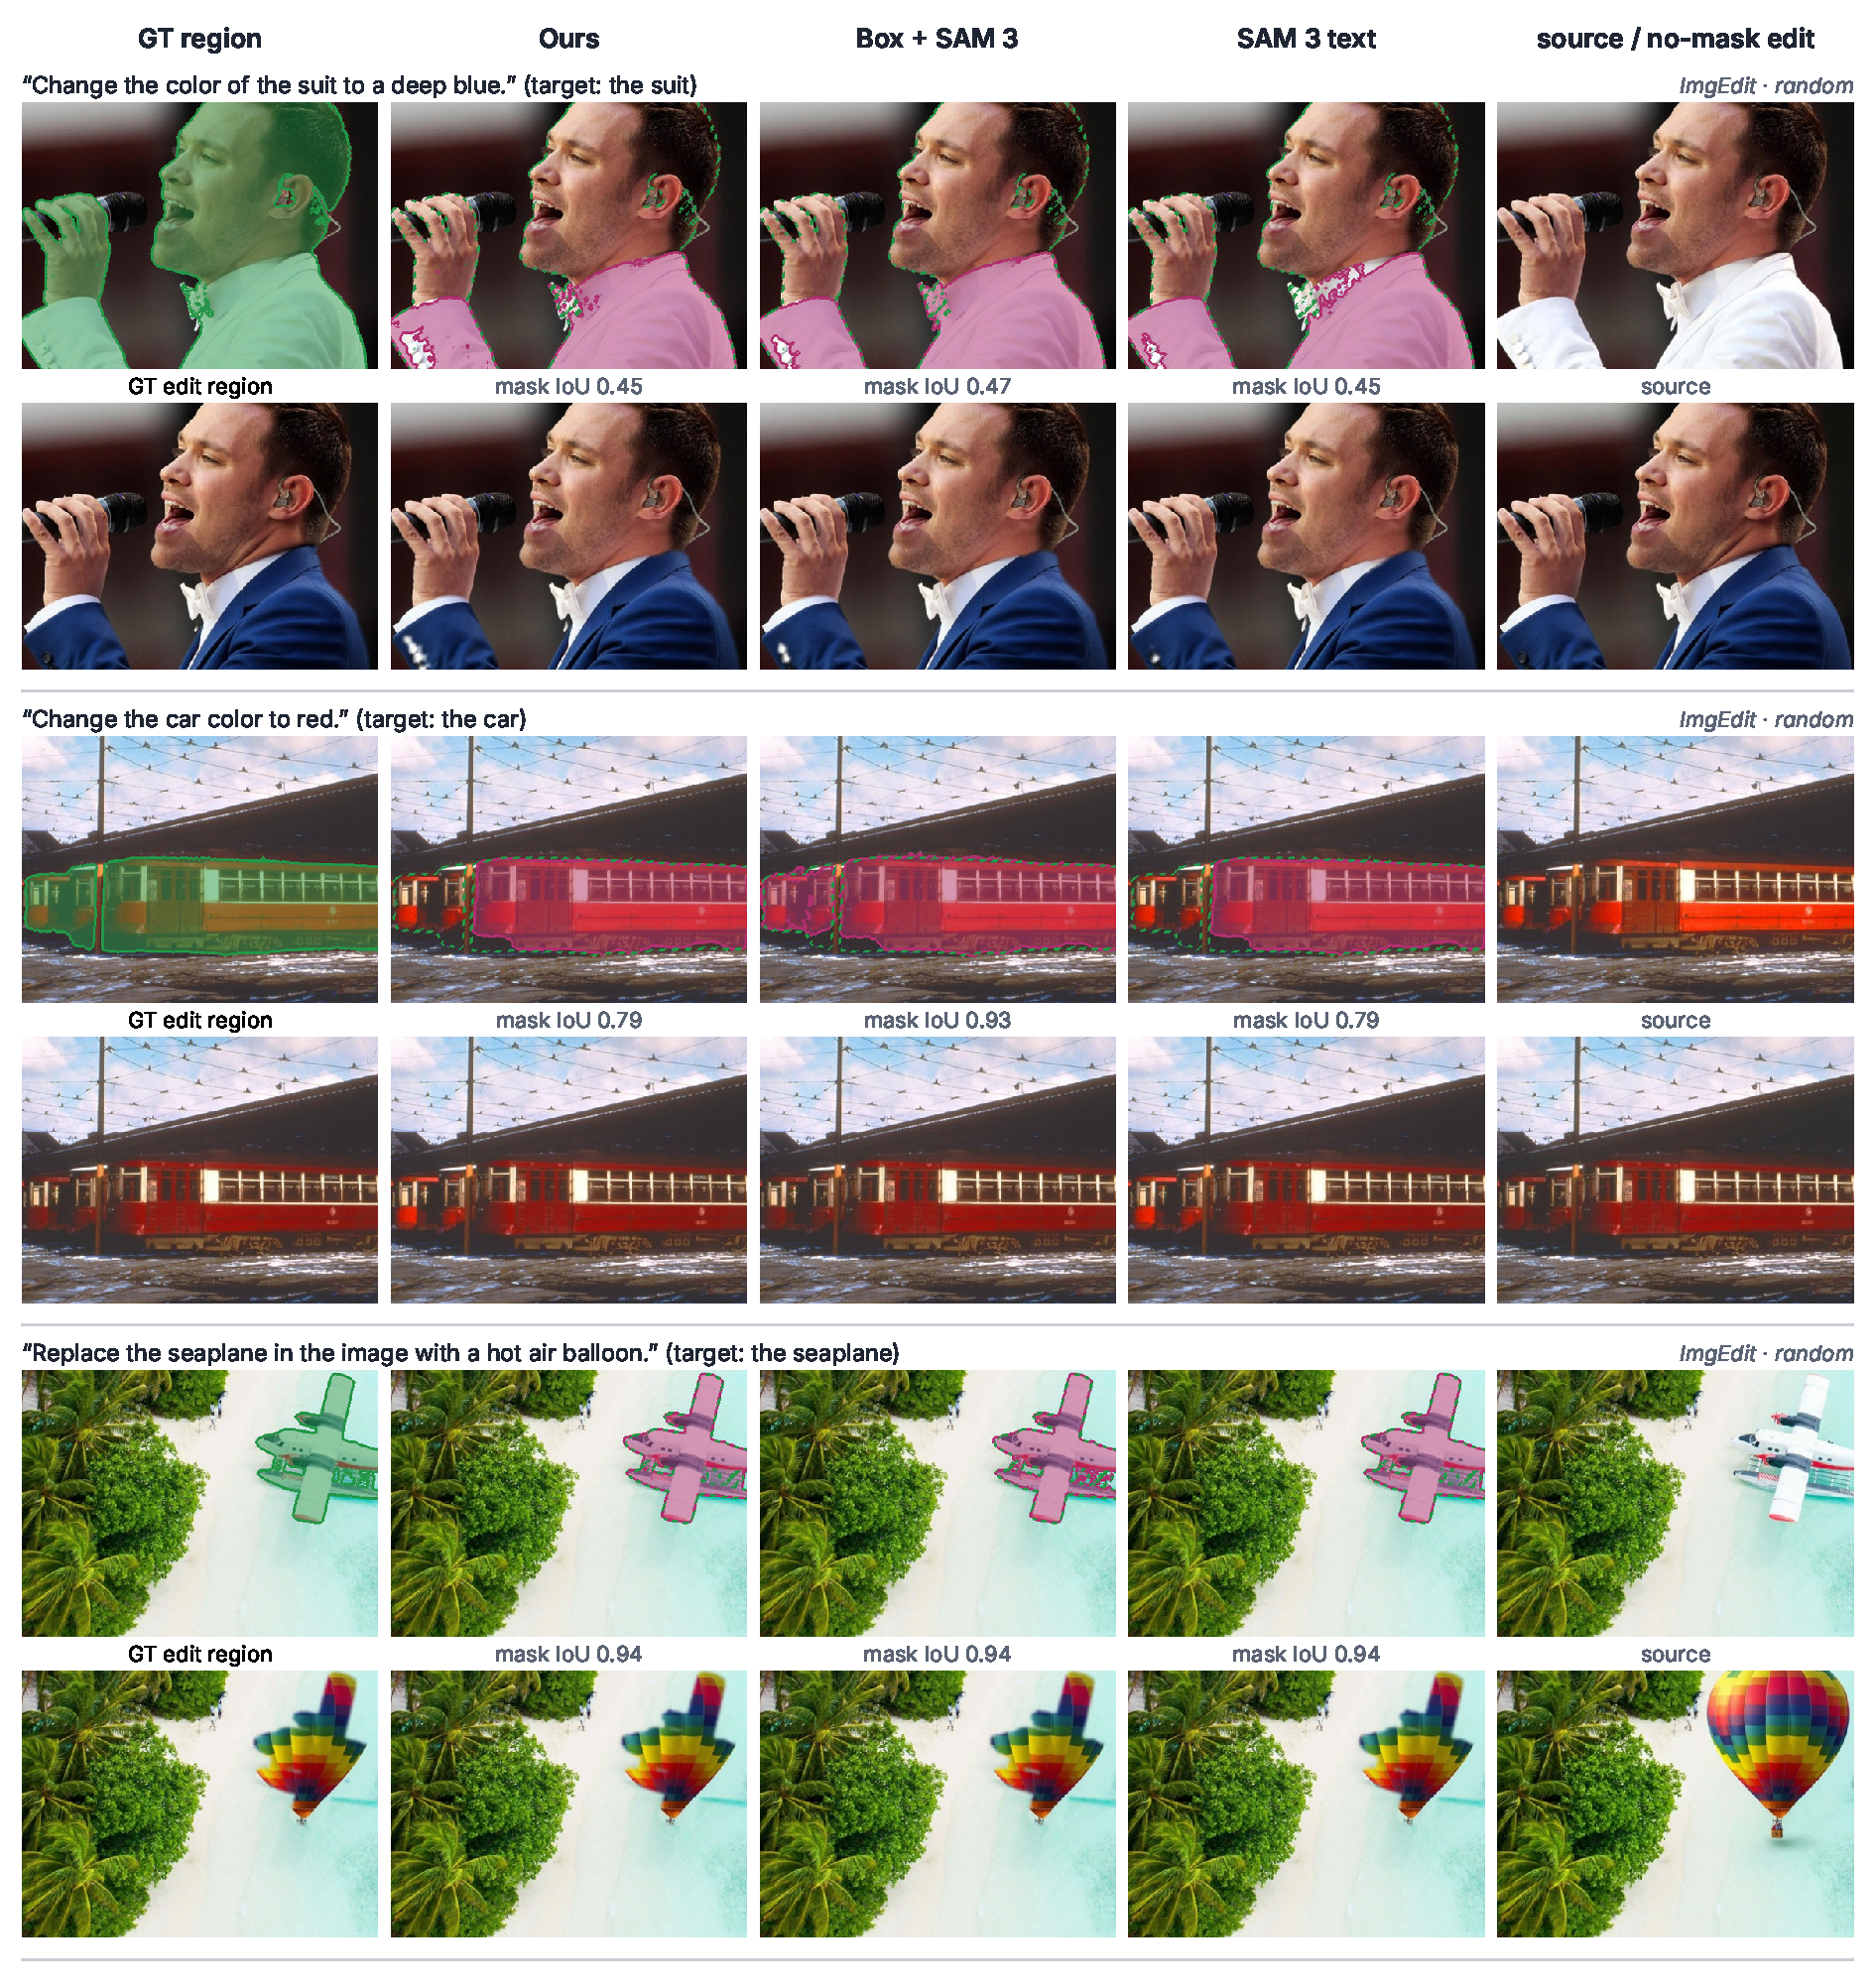
\includegraphics[width=\textwidth,height=0.92\textheight,keepaspectratio]{figures/qualitative/edit_imgedit_random.pdf}
\caption{\textbf{Editing, ImgEdit-Bench, Qwen-Image-Edit, random sample.} Top: masks of each source (GT edit region dashed); bottom: the edit within each mask and the unmasked edit.}
\label{fig:appx_edit_imgedit_random}
\end{figure*}

\begin{figure*}[p]
\centering
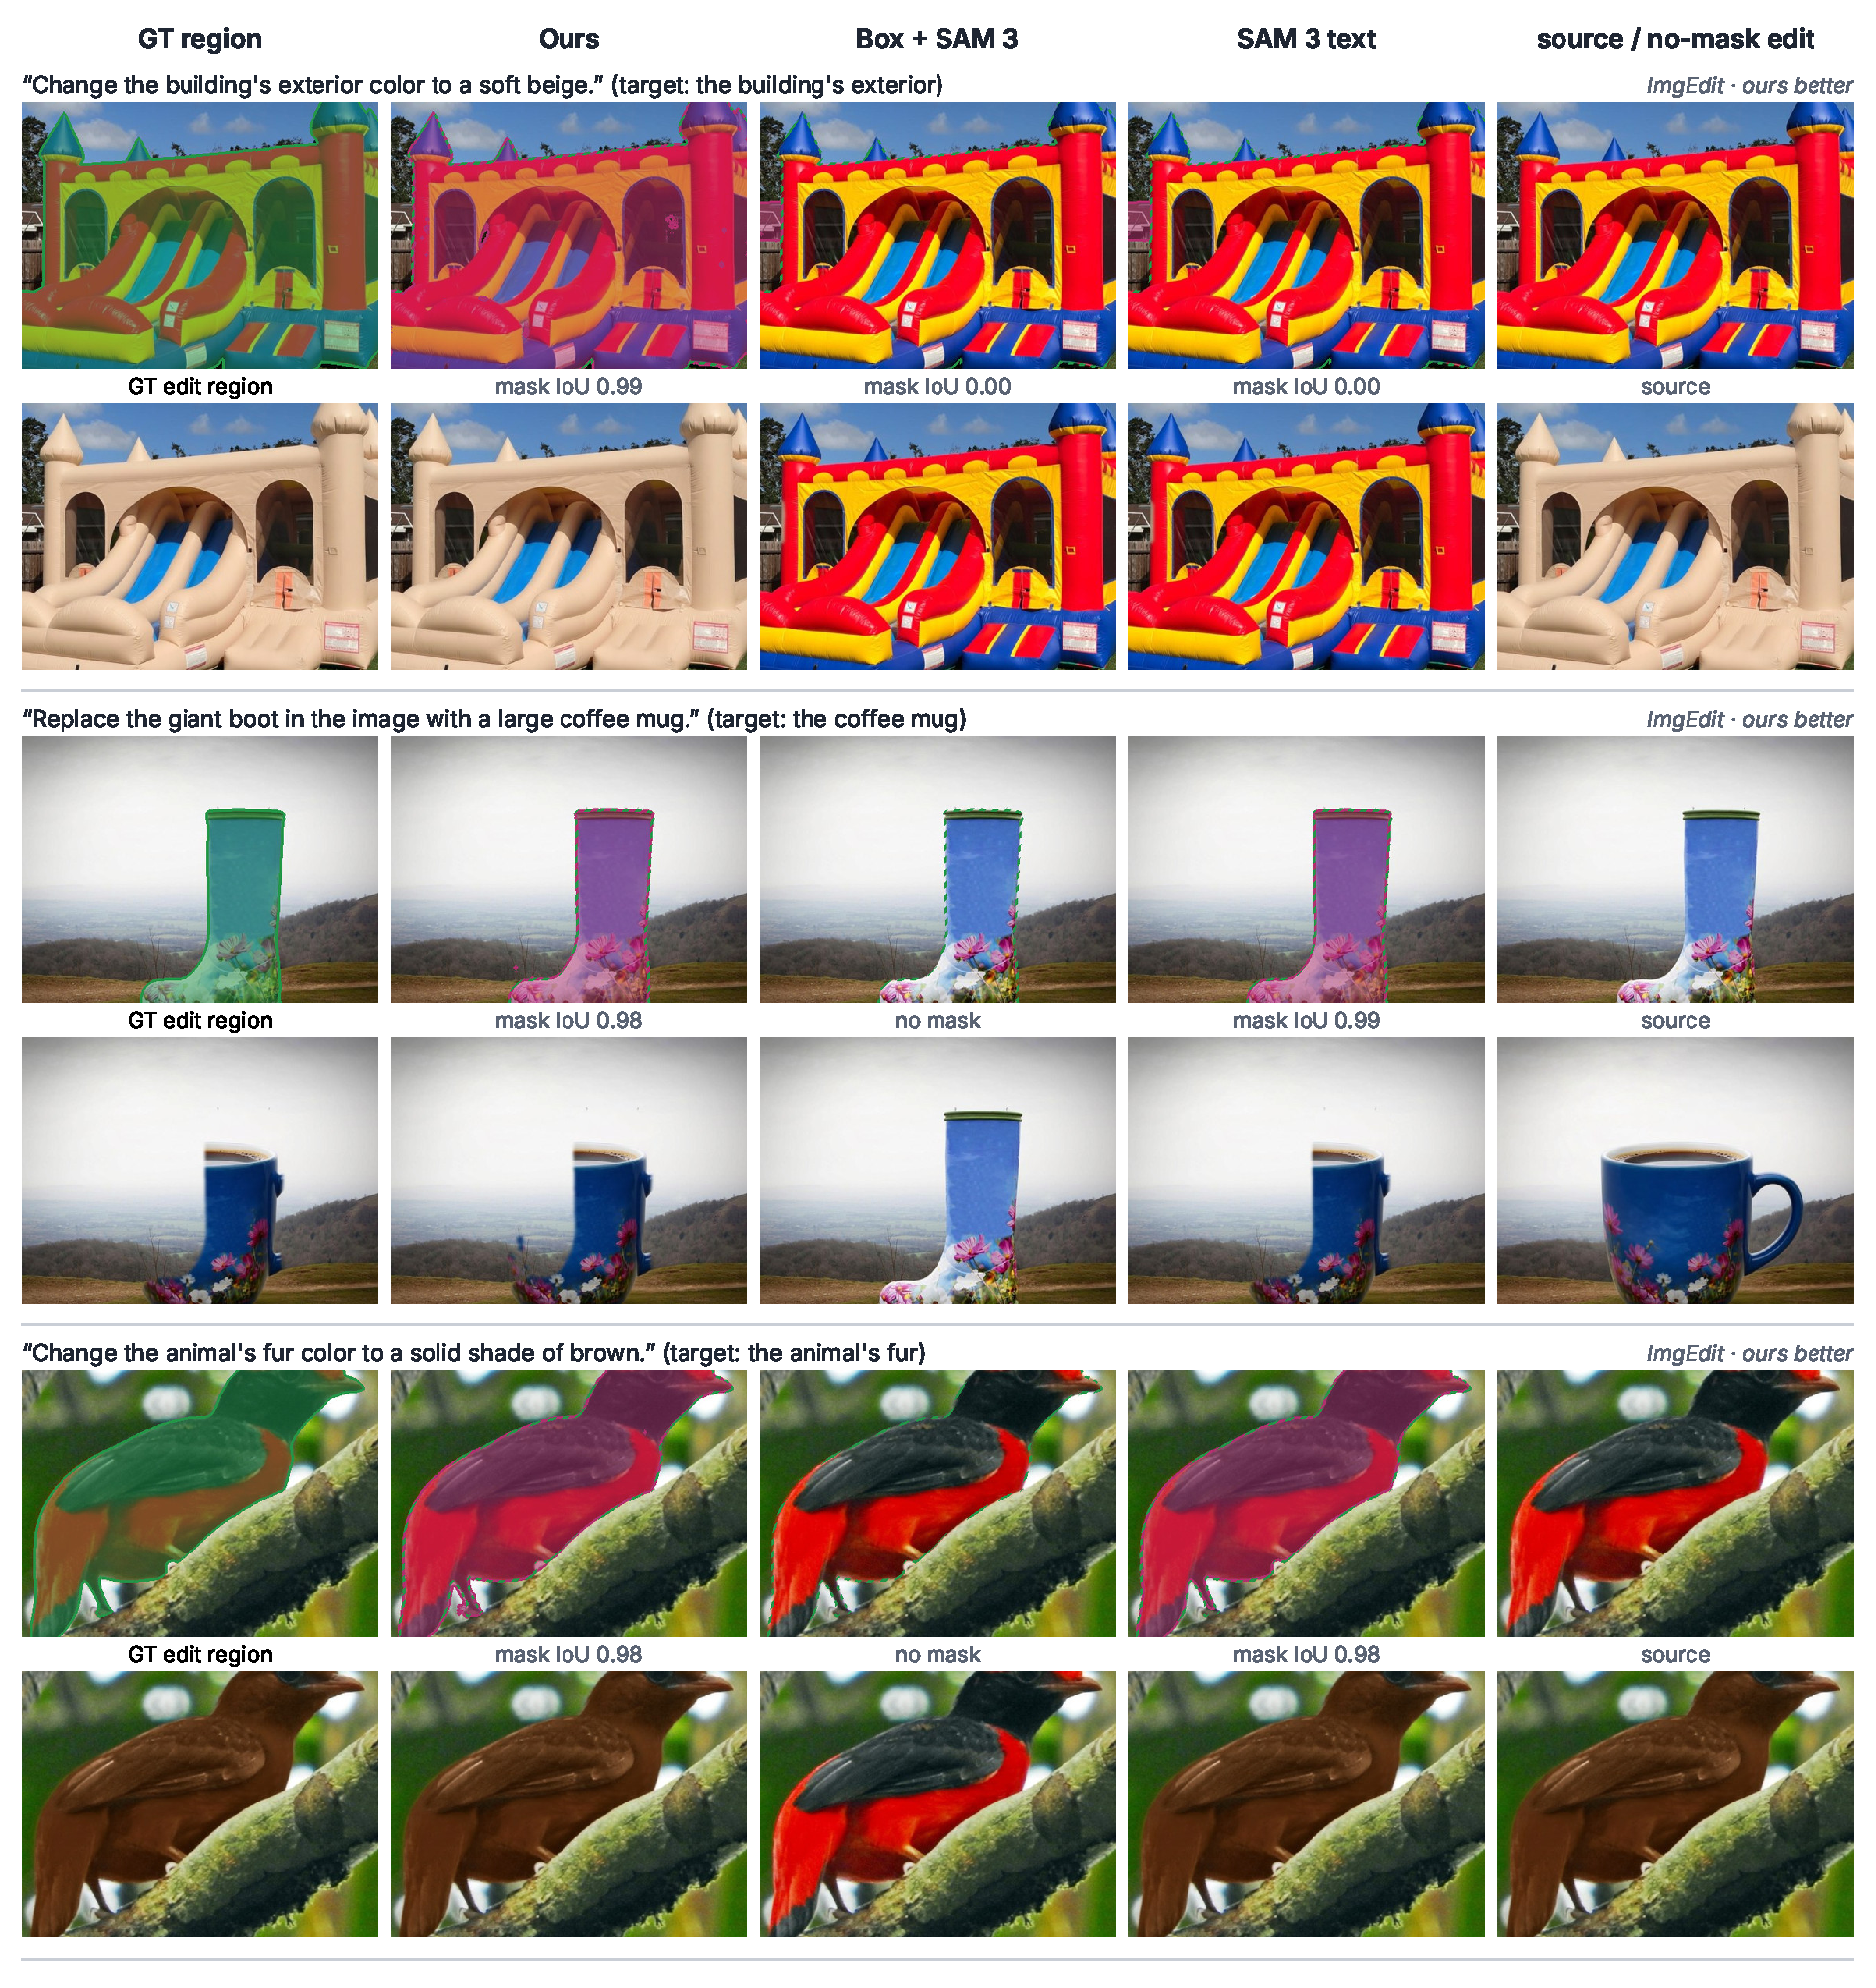
\includegraphics[width=\textwidth,height=0.92\textheight,keepaspectratio]{figures/qualitative/edit_imgedit_ours_better.pdf}
\caption{\textbf{Editing, ImgEdit-Bench, Qwen-Image-Edit, largest margins for \ours{}.} Top: masks of each source (GT edit region dashed); bottom: the edit within each mask and the unmasked edit.}
\label{fig:appx_edit_imgedit_ours_better}
\end{figure*}

\begin{figure*}[p]
\centering
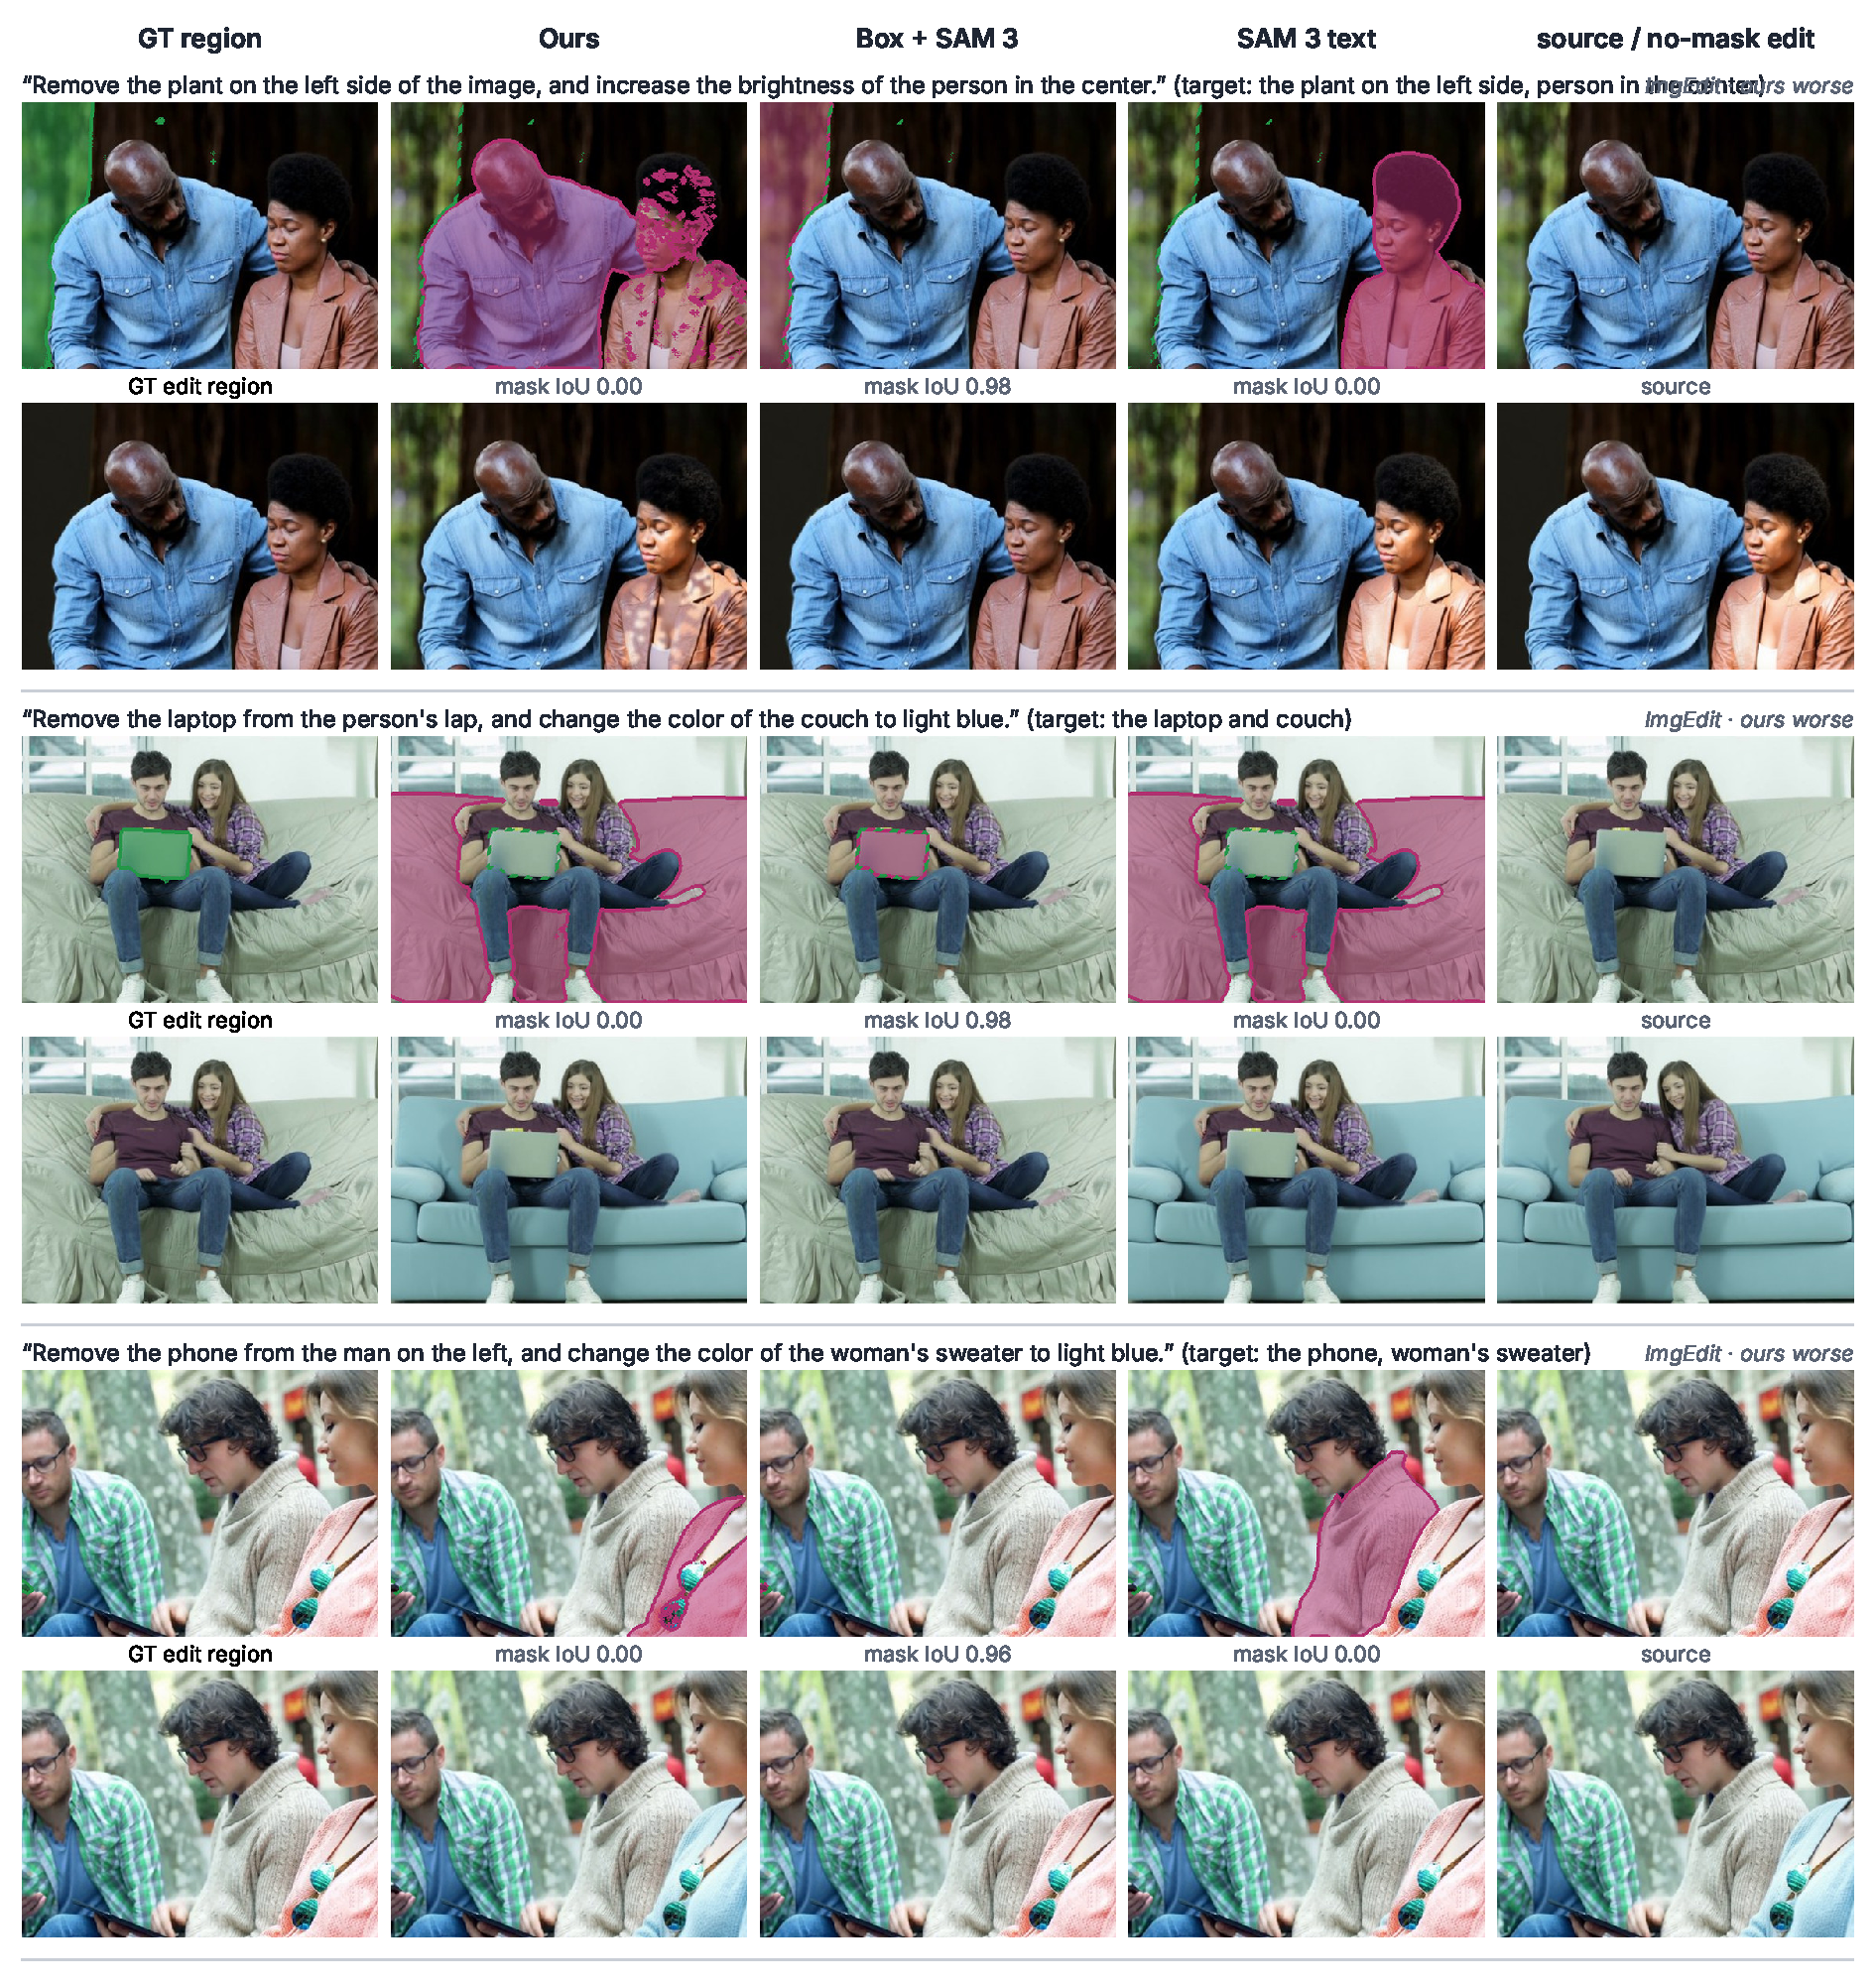
\includegraphics[width=\textwidth,height=0.92\textheight,keepaspectratio]{figures/qualitative/edit_imgedit_ours_worse.pdf}
\caption{\textbf{Editing, ImgEdit-Bench, Qwen-Image-Edit, largest margins against \ours{}.} Top: masks of each source (GT edit region dashed); bottom: the edit within each mask and the unmasked edit.}
\label{fig:appx_edit_imgedit_ours_worse}
\end{figure*}

\begin{figure*}[p]
\centering
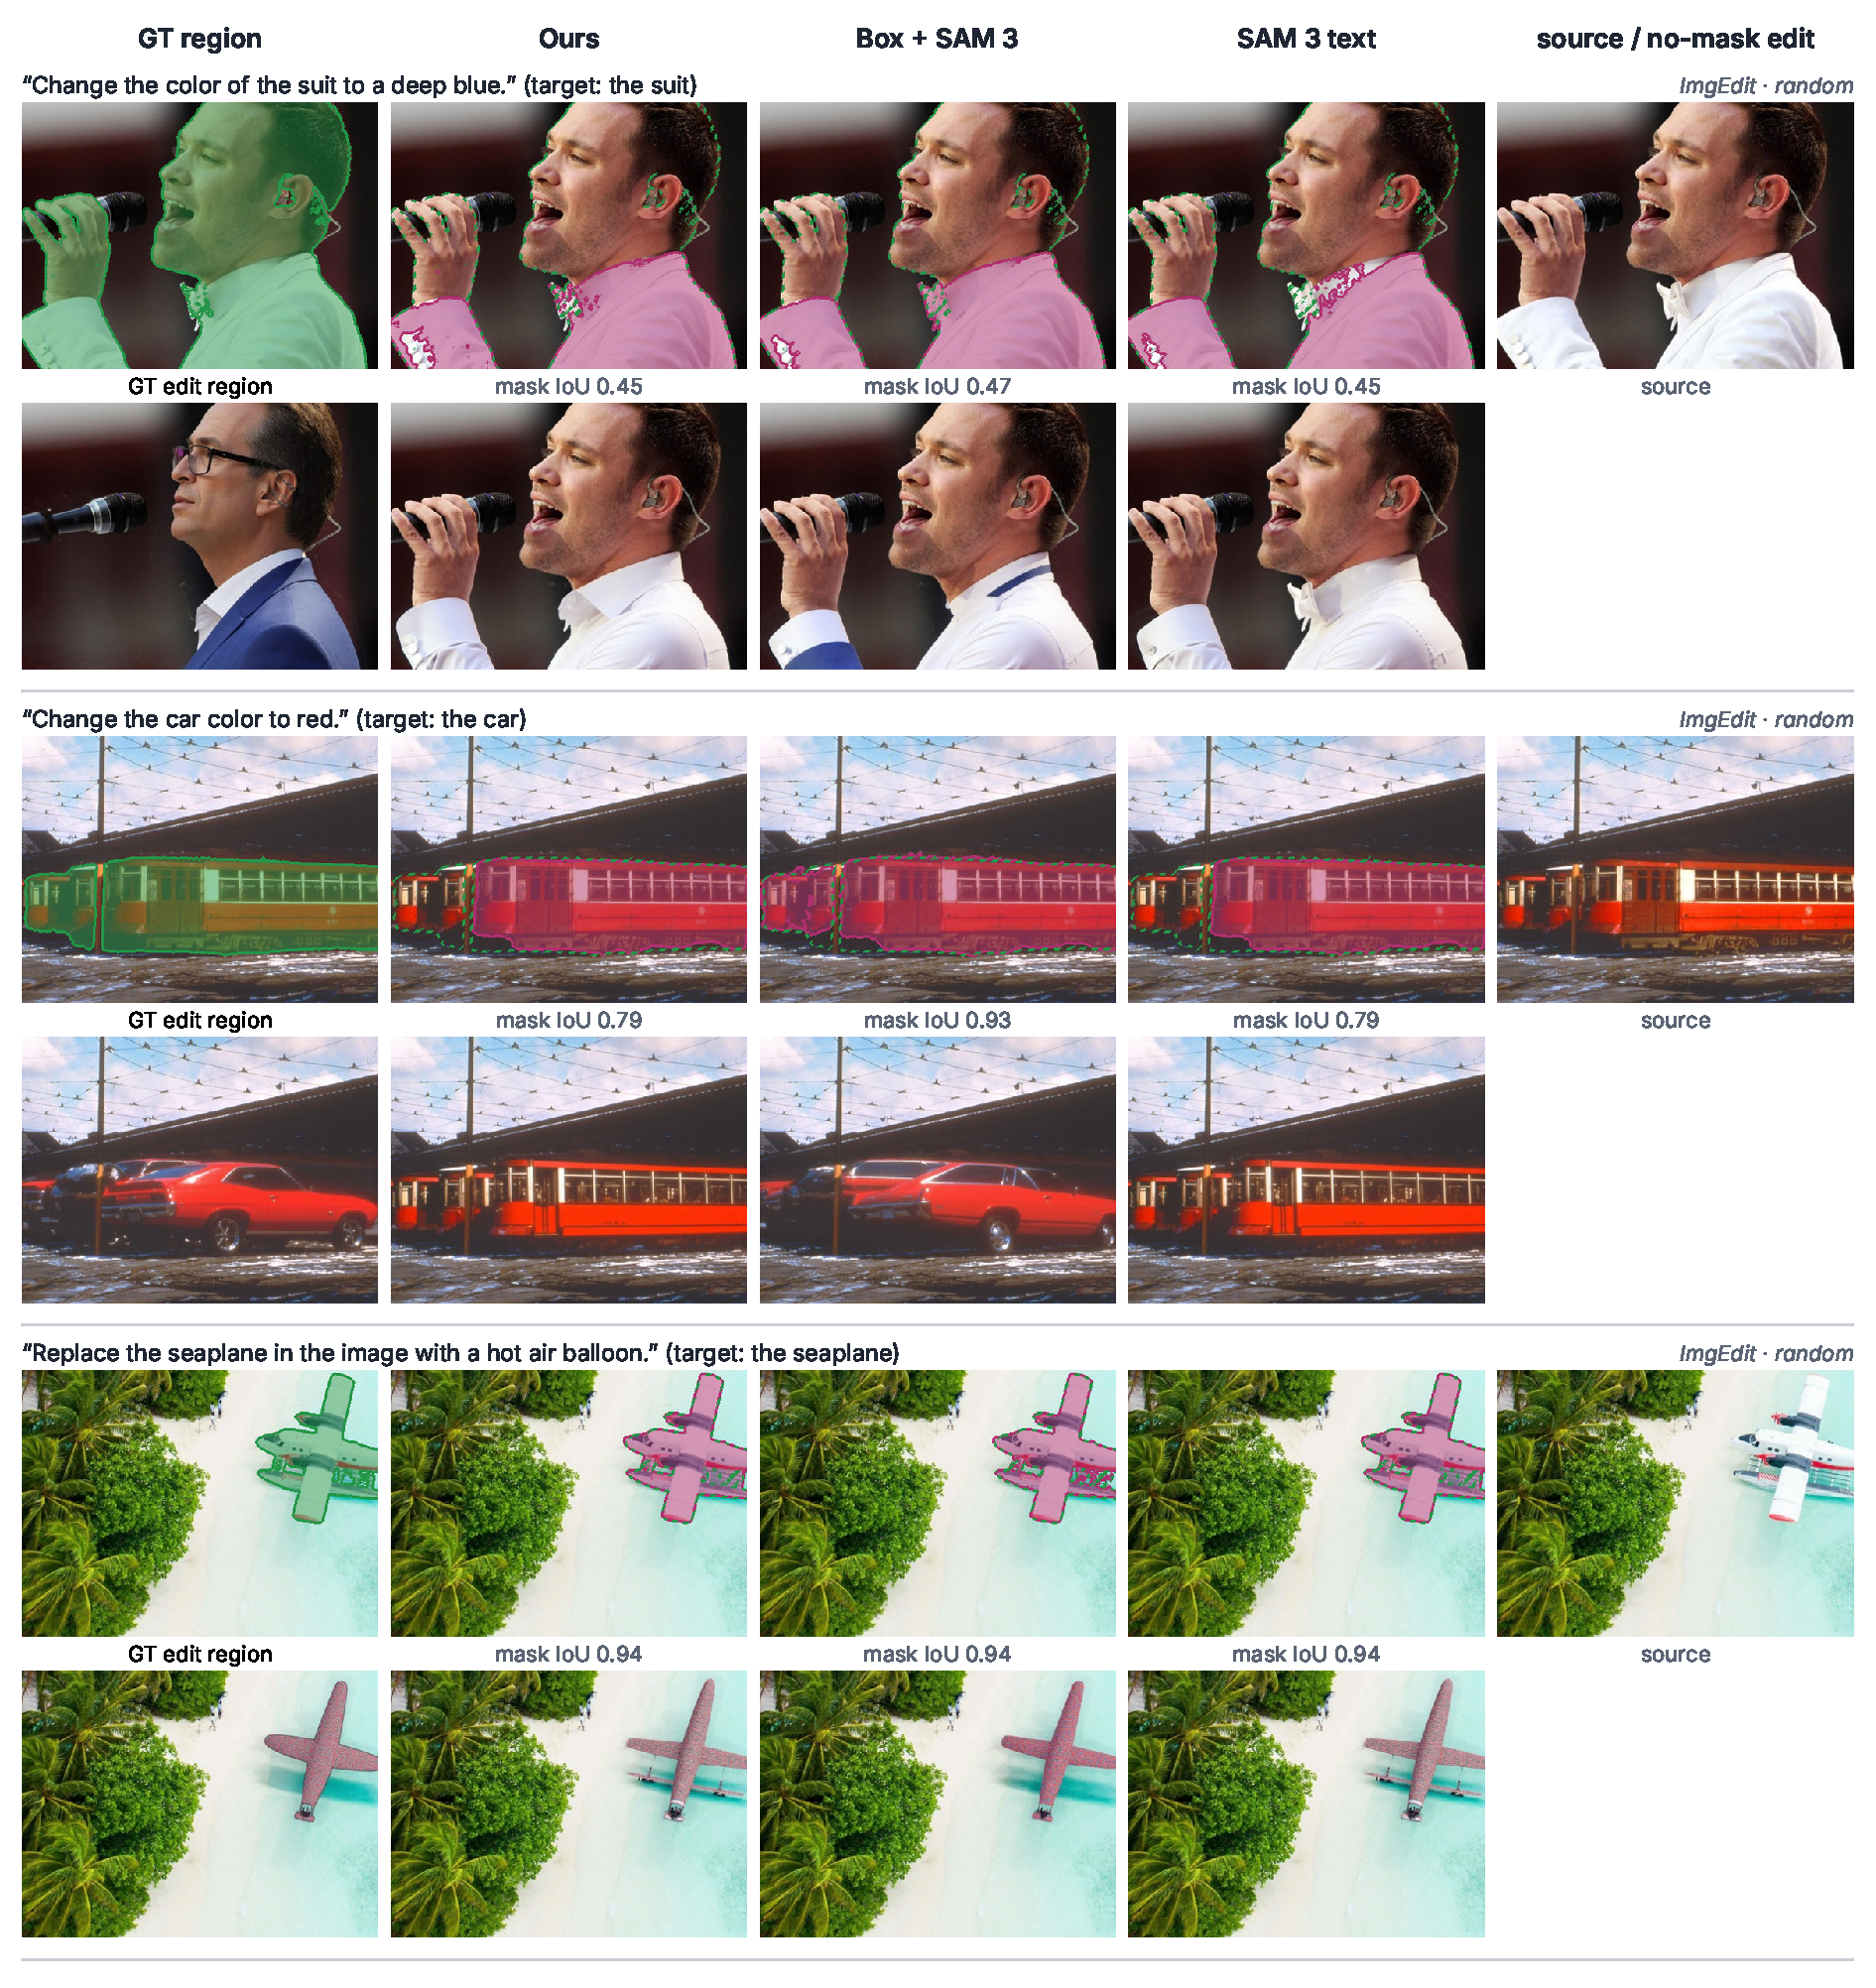
\includegraphics[width=\textwidth,height=0.92\textheight,keepaspectratio]{figures/qualitative/edit_imgedit_random_flux.pdf}
\caption{\textbf{Editing, ImgEdit-Bench, FLUX Fill, random sample.} As above, with FLUX Fill inpainting each mask.}
\label{fig:appx_edit_imgedit_flux}
\end{figure*}

